\documentclass[12pt]{article}

\usepackage{hyperref}
\hypersetup{
		colorlinks,
		citecolor=black,
		filecolor=black,
		linkcolor=black,
		urlcolor=black
	}

\usepackage[T2A]{fontenc}
\usepackage[utf8]{inputenc}
\usepackage[english,russian]{babel}

\usepackage{amsmath}
\usepackage{amsthm, mathrsfs, mathtools, amssymb}
\usepackage{enumitem}

\usepackage{epigraph}

\usepackage{tikz}
\usetikzlibrary{decorations.pathmorphing}
% для волнистой линии для фотонов создал стиль линии snake arrow
% рисует волну и на конце ее чуть-чуть прямую линию оставляет для стрелки
\tikzset{snake arrow/.style=
	{->,
		decorate,
		decoration={snake,amplitude=.4mm,segment length=2mm,post length=1mm}},
}
\usepackage{caption}
\usepackage{float}
\usepackage{multirow}
\usepackage{multicol}
\usepackage{wrapfig}
%\usepackage{hyperref}
%\hypersetup{
%	colorlinks,
%	citecolor=black,
%	filecolor=black,
%	linkcolor=black,
%	urlcolor=black
%}

\usepackage{geometry}
\geometry{verbose,a4paper,tmargin=1cm,bmargin=2cm,lmargin=1.5cm,rmargin=1.5cm}

\begin{document}
%  \tableofcontents \newpage
  
  \section{Письменная часть}
  
  \subsection{Спонтанное и вынужденное излучение. Вывести соотношение Эйнштейна для
коэффициентов A и B}\label{einstein-a-b}
%ref: M, 300
Пусть в полости с веществом, состоящем из одинаковых не взаимодействующих друг с
другом частиц, наблюдается термодинамическое равновесие. Для некоторой частицы с дискретным спектром энергий рассматриваем поведение при налетающем
(индуцирующим, в том плане, что оно вызывает вынужденное излучение) фотоне. Эта частица может
перейти на уровень выше, поглотив фотон, может перейти на уровень ниже, испустив
ещё один фотон вдобавок.
В случае испускания дополнительного фотона данное явление называется
\emph{вынужденным излучением}.

Также частица может самопроизвольно выпустить фотон, потеряв часть энергии и опустившись на
уровень ниже. Это явление называется \emph{спонтанным излучение}.

Обозначим $E_1, E_2$ --- энергии основного и возбужденного состояний\footnote{В
этой упрощённой модели, считаем, что больше уровней энергии нет.}, $N_1, N_2$ --- количество
частиц в основном и возбужденном состоянии. Тогда за некоторый промежуток $\Delta t$ произойдёт
какое-то количество переходов $\Delta n_{12}$ из состояния 1 в 2 и $\Delta n_{21}$ из
состояния 2 в 1.

Согласно распределению Ф-Д (Больцмана)
\[
  N_i \sim e^{-\dfrac{E_i}{kT}},\quad \frac{N_2}{N_1} = e^{-\dfrac{E_2 - E_1}{kT}},
\]
где $ k $ --- постоянная Больцмана.

Заметим что при данных условиях, излучение в полости монохроматическое с
частотой $ \omega $ такой, что $ E_2 - E_1 = \hbar\omega $. Для падающего излучения вспомним такую характеристику, как спектральная плотность излучения:
\[
  u_\omega = \dfrac{dW}{dV d\omega}.
\]
Она характеризует, если утрировать, количество фотонов в некотором элементе объёма.

\subsubsection{Случай отсутствия вынужденного излучения}
Предположим, что при налетающем фотоне может произойти только либо поднятие $1 \to 2$, 
либо просто как-то спонтанно произойти излучение $2 \to 1$. То есть предположим, что нет никакого
вынужденного излучения и это всё ложь.

Обозначим $z_{12}$ --- количество частиц, которые за единицу времени перейдут из 1 во
2-ое состояние, $z_{21}$ -- из 2 в 1. Ясно, что каждая из этих величин пропорциональна количеству
частиц на данном энергетическом уровне. Так же ясно, что частота переходов $1\to 2$, вызываемых
поглощением фотона, пропорциональна количеству налетаемых фотонов. Тогда:
\[
  \begin{cases}
    z_{12} = \dfrac{\Delta n_{12}}{\Delta t} \sim N_1 \cdot u_\omega, \\[10pt]
    z_{21} = \dfrac{\Delta n_{21}}{\Delta t} \sim N_2. 
  \end{cases}
  \Rightarrow
  \begin{cases}
    z_{12} = B_{12} N_1 u_\omega, \\
    z_{21} = A_{21} N_2.
  \end{cases}
\]
здесь коэффициенты $B_{12}$ и $A_{21}$ появились просто как константы
пропорциональности (вероятности переходов).
В термодинамическом равновесии за единицу времени в обе стороны переходит одинаковое количество 
частиц (принцип детального равновесия):
\begin{equation}\label{write_01:bad_einstein}
  z_{12} = z_{21} \Rightarrow
  B_{12} N_1 u_\omega = A_{21} N_2
  \Rightarrow
  B_{12} u_\omega = A_{21} \dfrac{N_2}{N_1}.
\end{equation}
Рассмотрим что будет происходить при нагреве $T \to \infty$, согласно распределению Ф-Д:
\[
  \dfrac{N_2}{N_1} = e^{- \dfrac{E_2-E_1}{kT}} \to 1,
\]
Из уравнения \eqref{write_01:bad_einstein} получаем, что:
\[
  \dfrac{A_{21}}{B_{12}}
  \approx u_\omega
  = \dfrac{\hbar \omega^3}{\pi^2 c^3} \cdot \dfrac{1}{e^{\dfrac{\hbar \omega}{kT}} - 1} \to \infty.
\]
(здесь использован закон Планка) получаем противорение -- не существует таких коэффициентов, чтобы
такая модель (без вынужденного излучения) работала.

\subsubsection{Случай вынужденного излучения}
Чтобы модель стала верной, надо добавить вынужденное излучнение. В этом случае к $z_{21}$ добавяться
ещё и частицы, которые выпустят фотон вследствие вынуждения:
\[
  \begin{cases}
    z_{12} = B_{12} N_1 u_\omega, \\
    z_{21} = A_{21} N_2 + B_{21} N_2 u_\omega.
  \end{cases}
\]
в термодинамическом равновесии за единицу времени в обе стороны переходит одинаковое количество 
частиц:
\begin{equation}\label{write_1:good_einstein}
  z_{12} = z_{21} \Rightarrow
  B_{12} N_1 u_\omega = A_{21} N_2 + B_{21} N_2 u_\omega
  \Rightarrow
  B_{12} \dfrac{N_1}{N_2} = \dfrac{A_{21}}{u_\omega} + B_{21}.
\end{equation}
При $T \to \infty$:
\[
  \dfrac{N_1}{N_2} = e^{- \dfrac{E_2-R_1}{kT}} \to 1,
  \dfrac{1}{u_\omega} = \dfrac{\pi^2 c^3}{\hbar \omega^3} \left(e^{\dfrac{\hbar \omega}{kT}} - 1\right) \to 0
  \Rightarrow
  \begin{cases}
    B_{12} = B_{21} = B, \\
    A_{21} = A 
  \end{cases}
\]
Таким образом:
\begin{multline*}
  B N_1 u_\omega = A N_2 + B N_2 u_\omega
  \Rightarrow
  B u_\omega \left( \dfrac{N_1-N_2}{N_2} \right) = A
  \Leftrightarrow \\
  \Leftrightarrow
  B u_\omega \left( \dfrac{N_1}{N_2} - 1 \right) = B u_\omega \left( e^{\dfrac{E_2-E_1}{kT}} - 1 \right) = A
  \Leftrightarrow
  B \dfrac{\hbar \omega^3}{\pi^2 c^3} = A
\end{multline*}
Последнее называется соотношением Эйнштейна.
 \newpage
  \subsection{Сформулировать квантовомеханическую задачу для гармонического осциллятора. Получить
его решение. Указать, на каком этапе решения возникает квантование энергии. Правила отбора
для гармонического осциллятора.}
Рассмотрим гармонические колебания в одномерном случае. В классической физике
имеем\footnote{Понятно, что в реальности такой силы сущестовать не может и
рассмотрение ограничивается приближёнными малыми колебаниями.} $ F_x = -kx $, и, значит,  
\begin{equation}
    U(x) = \frac{kx^2}{2} = \frac{m_0\omega_0^2 x^2}{2},
    \label{eq:potenc}
\end{equation}
где $ \omega_0^2 = k/m_0 $ --- квадрат собственной частоты классического
гармонического осцилятора. Таким образом, рассматривается движение частицы в
параболической потенциальной яме. 
\begin{figure}[h]
  \centering
  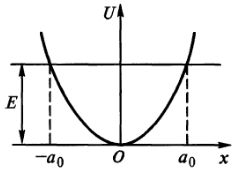
\includegraphics[width=0.3\textwidth]{img/write-02/yama.png}
  \caption{Потенциальная энергия гармонического осциллятора.}
  \label{fig:yama}
\end{figure}
На рисунке \ref{fig:yama} число $ a_0 $ есть, конечно,
амплитуда колебаний. Считая без потери общности движение равным $ x = a_0 \cos\omega t $, легко
получим 
\[
    E = \frac{m_0a_0^2\omega_0^2}{2}, \quad a_0 =
    \sqrt{\frac{2E}{m_0\omega_0^2}}.
\]

Перейдём к квантовому случаю. А именно, решим уравнение Шрёдингера
для потенциальной энергии \eqref{eq:potenc}: 
\[
    \frac{\hbar^2}{2m} \psi''(x) + \left(E - \frac{kx^2}{2}\right) \psi(x) = 0.
\]

\subsubsection{Решение уравнения}
\textbf{1. Масштабирование}. Перейдём к безразмерным величинам $ \varepsilon =
E/E_0 $, $ \xi = x/x_0 $. Здесь $ E_0 = E_{\min} = \hbar \omega/2 = kx_0/2 $.
Обоснуем: 
\begin{align*}
  \Delta x &= \sqrt{\langle x^2\rangle} = \sqrt{\frac{1}{2} a_0^2} =
  \sqrt{\frac{E}{m_0\omega_0^2}},\\
  \Delta p &= \sqrt{\langle p^2 \rangle} =
  \sqrt{\frac{1}{2}m_0^2a_0^2\omega_0^2} = \sqrt{m_0E},
\end{align*}
откуда вместе с неравенством Гейзенберга $ \Delta x \Delta p \geqslant \hbar/2 $
и следует результат. Итак, перейдём к величинам $ \varepsilon $, $ \xi $ и
получим уравнение
\begin{equation}
  \psi'' + (\varepsilon - \xi^2)\psi = 0.  
  \label{eq:eq1}
\end{equation}

\textbf{2. Асимптотика.} Устремим в уравнении $ |\xi| \to \infty $. Тогда
главная часть примет вид 
\[
    \psi'' = \xi^2 \psi.
\]
Хорошо бы $ \psi \to 0 $, откуда вытекает предположение о виде волновой функции
$ \psi = e^{\alpha(\xi)} $, где $ \alpha(\xi) \to -\infty $. Тогда $ \psi'' =
(\alpha'' + (\alpha')^2)e^\alpha $, а значит, $ \alpha'' + (\alpha') = \xi^2 $.
Тогда (?) $ \alpha = A\xi^n $. В этом предположении в связи с рассматриваемой
асимптотикой будем рассматривать только слагаемое в квадрате, получим $
A^2n^2\xi^{2n-2} \approx \xi^2 $, откуда $ A = -1/2 $, $ n= 2 $. Искомая
асимптотика --- $ \psi  \to \exp( - \xi^2/2) $.

\textbf{3. Общий вид.} Будем в таком случае искать решение в виде $ \psi(\xi) =
\exp(-\xi^2/2)f(\xi)$. Подставив в \eqref{eq:eq1} и упростив выражение, получим 
\begin{gather*}
    \psi'' = \exp(-\xi^2/2)^{(2)}f + 2\exp(-\xi^2/2)^{(1)}f^{(1)} +
    \exp(-\xi^2/2) f^{(2)} = \exp(-\xi^2/2)(f''-2\xi f' + (\xi^2 - 1)f),\\
    f'' - 2\xi f' + (\varepsilon - 1)f = 0.
\end{gather*}
Саму функцию $ f $ представим рядом $ f = \sum\limits_{k=0}^{+\infty} a_k
\xi^k$. Тогда  
\begin{align*}
  f' &= \sum_{k=0}^\infty ka_k \xi^{k-1},\\
  f'' &= \sum_{k=0}^\infty k(k-1) a_k
  \xi^{k-2} = \sum_{k=0}^\infty (k+1)(k+2) a_{k+2}\xi^k.
\end{align*}
Получаем для любого $ \xi $  
\[
  \sum_{k=0}^\infty ((k+2)(k+1)a_{k+2} + (-2k + \varepsilon - 1) a_k)\xi^k = 0.
\]
Благодаря произвольности $ \xi $ можем вывести теперь рекуррентное соотношение 
\begin{equation}
  a_{k+2} = \frac{2k+1-\varepsilon}{(k+2)(k+1)}a_k \approx \frac{2}{k}a_k
  \label{eq:rek}
\end{equation}
при $ k \to \infty $. С другой стороны для некоторого $ k' = k/2 $
\[
  \exp(\xi^2) = \sum_{k'=0}^\infty \frac{\xi^{2k'}}{k'!} = \sum_{k=0}^\infty
  \frac{\xi^k}{(k/2)!},
\]
где для последнего ряда также выполняется предельное рекуррентное соотношение
\eqref{eq:rek}. Поэтому и примем $ f(\xi) = \exp(\xi^2) $. Однако в этом случае
$ \psi = \exp(\xi^2/2) \to \infty $ при $ \xi \to \infty $.

\textbf{4. Квантование.} Приходим к тому, что ряд $ f(\xi) $ нужно оборвать.
Рассмотрим индекс последнего ненулевого члена $ n := k_{\max} $ и нулевой член $ a_{n+2} $. Из реккурентного
соотношения \eqref{eq:rek} вытекает теперь, что $ \varepsilon = 2n+1 $. Заметим,
что этот факт и говорит о квантовании энергии. Сама энергия имеет вид
\[
  E_n =
  \frac{\hbar \omega_0}{2} + n\hbar\omega_0.
\]

\textbf{5. Полиномы Чебышёва -- Эрмита.} Получили, что $ f(\xi) $ есть некие
полиномы степени $ n $. Конкретный вид полиномов выберем из соображений
ортогональности решений. Ими будут полиномы Эрмита  
\[
  H_n := (-1)^n \exp(x^2) \frac{d^n}{d\xi^n}\exp(-x^2),
\]
которые как раз имеют
\emph{вес} $ \exp(-\xi^2) $, то есть 
\[
  \int\limits_{-\infty}^{\infty}H_n H_m \exp(-\xi^2)\,d\xi =
  \frac{\delta_{nm}}{A_nA_m},
\]
где коэффициент 
\[
  A_k = \frac{1}{\sqrt{2^kk!\sqrt{\pi}}}.
\]

Таким образом, волновые функции будут равны 
\[
    \psi_n(\xi) = A_n \exp(-x^2/2) H_n(\xi).
\]
\qed

\begin{figure}[h]
  \centering
  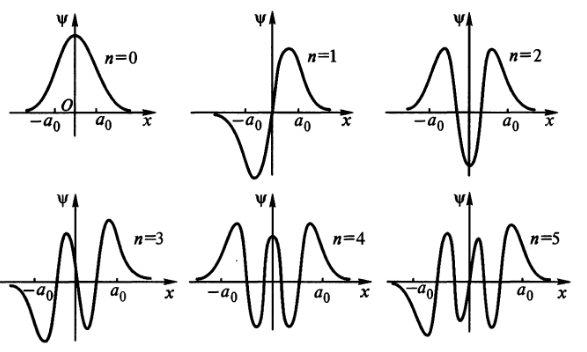
\includegraphics[width=0.8\textwidth]{img/write-02/psi.png}
  \caption{Волновые функции гармонического осциллятора}
  \label{fig:psi}
\end{figure}

Обратим внимание, что энергия, а значит, амплитуда $ a_0 $ зависят от $ n $. При
этом в отличие от прямоугольных ям энергия с переходом на новый уровень меняется
на равные отрезки $ \Delta E = \hbar\omega_0 $. Точный расчет
показывает, что особенности испускания и поглощения 
электромагнитного излучения гармоническим осциллятором таковы, что 
возможны переходы только между соседними уровнями. Условия, которые определяют
изменение квантовых чисел при разрешенных переходах системы из одного состояния в другое,
называются правилами отбора. Таким образом, согласно правилам
отбора, квантовое число $ n $ при испускании и поглощении 
электромагнитного излучения квантовым гармоническим осциллятором
может изменяться только на единицу.

Снова минимальная энергия положительна, что играет очень важную роль в физике (см., напр.,
отсутствие кристаллизация гелия при абсолютном нуле и нормальном давлении).

Попробуем рассчитать вероятность для классического осциллятора. Там $ x =
a_0\sin \frac{2\pi}{T}t $, $ dx = a_0 \frac{2\pi}{T} \cos \frac{2\pi}{T}t\,dt $,
и вероятность $ dP $ того, что
частица при движении в одну сторону находится в интервале шириной $ dx $,
равна 
\[
  dP = \frac{dt}{T/2} = \frac{dx}{\pi\sqrt{a_0^2 - x^2}}.
\]
При больших $ n $ функция $ |\psi_n|^2 $ похожа на $ dP/dx $, однако для малых
$ n $ они отличаются очень сильно.

\begin{figure}[h]
  \centering
  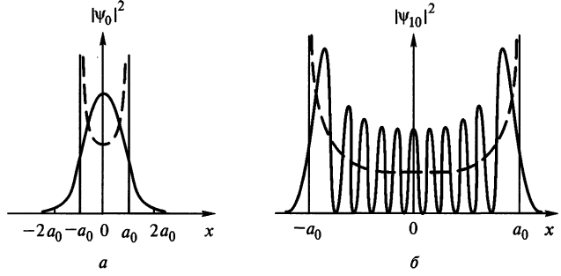
\includegraphics[width=0.8\textwidth]{img/write-02/dPdx.png}
  \caption{Плотности вероятности обнаружения частицы для 
квантового (сплошная линия) и классического (пунктирная линия) осциллятора.}
  \label{fig:dPdx}
\end{figure}
 \newpage
  \subsection{Записать операторные уравнения для проекции момента импульса $L_z$ и для квадрата момента
импульса $L^2$. Получить решение уравнения для $L^2$. Показать, что из условия однозначности
и конечности $\psi$-функции следует квантование величин $L_z$ и $L^2$ }


 \newpage
  \subsection{Записать уравнение Шрёдингера для атома водорода в сферических координатах и произвести
разделение переменных. Решить уравнение для радиальной части $R(r)$ волновой функции. Показать,
что из решения уравнения для $R(r)$ при выполнении условий регулярности следует дискретность
энергии атома водорода.}


 \newpage
  \subsection{Сформулировать, какие частицы называются фермионами, привести примеры Ферми-частиц.
Сформулировать принцип Паули (W. Pauli). Используя формулу Больцмана для энтропии, вывести
распределение Ферми-Дирака}

Про фермионы см. \ref{princip-nerazlichimosti}.

\paragraph{Принцип Паули}
\textit{Системы электронов (фермионов) встречаются в природе только в состояниях, описываемых антисимметричными волновыми функциями. }

Отсюда следует, что два одинаковых электрона (фермиона), входящих в одну систему, не могут находиться в одинаковых состояниях (иначе при перестановке волновая функция была бы чётной)\footnote{Однако отметим, что в одинаковом состоянии может находиться любое число бозонов.}.

\paragraph{Другая формулировка} В одном и том же атоме не может быть более одного электрона с одинаковым набором четырёх квантовых чисел $n, l , m, m_s$ (про квантовые числа также см. \ref{princip-nerazlichimosti}).

\paragraph{Вывод распределения Ферми-Дирака}
Рассмотрим идеальный ферми-газ, то есть систему, состоящую из $N$ невзаимодействующих фермионов.
\begin{figure}[H]
	\centering
	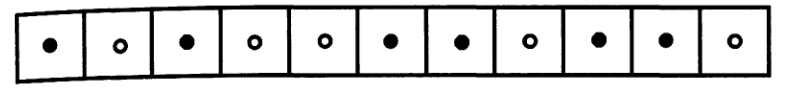
\includegraphics[width=0.7\linewidth]{img/write-05/yacheiki}
	\caption{Возможное распределение ферми-частиц по ячейкам (черная точка - ферми частица, белая точка - отсутсвие частицы)}
	\label{fig:yacheiki}
\end{figure}
Разбив систему на $Z$ ячеек, найдем количество распределений $N$ фермионов по $Z$ ячейкам, то есть статистический вес макросостояния системы фермионов
\begin{equation*}
	W = \frac{Z!}{N!(Z-N)!}
\end{equation*}

Рассмотрим шестимерное фазовое пространство с координатами $x,y,z,p_x,p_y,p_z$. Разобьем его с помощью изоэнергетических поверхностей
\begin{equation*}
	f(x,y,z,p_x,p_y,p_z) = E_i = \mathrm{const}
\end{equation*}
на тонкие слои так, что $|E_{i+1}-E_{i}|\ll E_i$. Пусть в пределы $i$-го слоя попадает $Z_i$ ячеек объемом $(2\pi\hbar)^3$ и $N_i$ частиц. Тогда аналогично примеру с раскладыванием фермионов по ячейкам получим статистический вес каждого энергетического слоя:
\begin{equation*}
	\Omega_i = \frac{Z_i!}{N_i!(Z_i-N_i)!}
\end{equation*}
Статистический вес всей системы равен произведению статистических весов её подсистем:
\begin{equation*}
	\Omega = \prod_i \Omega_i
\end{equation*}

Для нахождения наиболее вероятного распределения частиц по ячейкам, необходимо найти максимум статистического веса системы при условии, что количество частиц постоянно и полная энергия постоянна (жесткая адиабатическая оболочка), то есть
\begin{equation*}
	\sum N_i=\mathrm{const},\quad \sum E_iN_i=\mathrm{const}.
\end{equation*}

Вспомним формулу Больцмана для энтропии $S=k\ln \Omega$, вместо максимума $\Omega$ будем искать максимум энтропии. По свойствам логарифмов:
\begin{equation*}
	S=k\sum_i \big[\ln Z_i! - \ln N_i ! - \ln(Z_i - N_i)!\big]
\end{equation*}

Так как $N_i, Z_i \gg 1$, то воспользуемся формулой Стирлинга ($\ln n! \approx n\ln n - n$).
\begin{equation*}
	S=k\sum_i \big[
	Z_i \ln Z_i - Z_i - N_i \ln N_i + N_i - (Z_i-N_i)\ln(Z_i-N_i) + (Z_i-N_i)
	\big]
\end{equation*}
Слагаемое $Z_i \ln Z_i$ исключим из выражения, так как при поиске экстремума энтропии варьироваться будут только числа частиц в слое $N_i$, а данное слагаемое от них не зависит.

\textit{Метод множителей Лагранжа}. Рассмотрим функцию
\begin{equation*}
	F = S + \lambda_1 N + \lambda_2 E = -k\sum_i \big[N_i\ln N_i+(Z_i-N_i)\ln (Z_i-N_i)\big] + \lambda_1 \sum_i N_i + \lambda_2 \sum_i N_iE_i
\end{equation*}
Приравнивая к нулю частные производные $F$ по $N_i$, получаем:
\begin{equation*}
	\frac{\partial F}{\partial N_i} = -k \left[
	\ln N_i + N_i\frac{1}{N_i}-\ln(Z_i-N_i)-(Z_i-N_i)\frac{1}{Z_i-N_i}
	\right] + \lambda_1 + \lambda_2 E_i = k \ln \frac{Z_i-N_i}{N_i} + \lambda_1 + \lambda_2E_i=0
\end{equation*}
Отсюда следует, что:
\begin{equation*}
	\ln \frac{Z_i-N_i}{N_i} = -\frac{\lambda_2 E_i+\lambda_1}{k} \Leftrightarrow
	\frac{Z_i-N_i}{N_i} = \frac{1-\frac{N_i}{Z_i}}{\frac{N_i}{Z_i}}=\exp \left\{-\frac{\lambda_2 E_i+\lambda_1}{k}\right\}
\end{equation*}
Отношение $\frac{N_i}{Z_i}$ представляет собой среднее число фермионов $<n_i>$ в одной ячейке (т.е. в одном квантовом состоянии). Наиболее вероятным значением $<n_i>$, как следует из поиска экстремума, является:
\begin{equation*}
	<n_i>=\frac{1}{\exp \left\{-\frac{\lambda_2 E_i+\lambda_1}{k}\right\}+1}
\end{equation*}

Поскольку все частные производные $F$ по $N_i$ равны нулю, то равен нулю и дифференциал этой функции $dF$, то есть:
\begin{equation*}
	dF = dS + \lambda_1 dN + \lambda_2 dE = 0
\end{equation*}
Но так как число частиц системы постоянно ($\sum N_i=\mathrm{const}$), то $dN=0$, а следовательно:
\begin{equation*}
	dS + \lambda_2 dE = 0 \implies \lambda_2 = -\frac{dS}{dE}
\end{equation*}
\begin{equation*}
	\begin{cases}	
	dS \overset{\mathrm{def}}{=\joinrel=} \frac{\delta Q}{T}\\
	\delta Q = dE,\,\text{т.к.}\, V=\mathrm{const}
	\end{cases}\implies \lambda_2 = -\frac{dS}{dE} = -\frac{\delta Q}{TdE} = -\frac{1}{T}
\end{equation*}
Множитель $\lambda_1$ представим в виде $\lambda_1=\frac{\mu}{T}$, где $\mu$ - некоторая функция параметров состояния системы, в частности температуры. $\mu$ называют химический потенциал.

С учетом выражений для $\lambda_1,\,\lambda_2$, освобождаясь от индекса $i$, получаем
\begin{equation*}
	<n>_{\textsc{Ф-Д}}=\frac{1}{\exp \left\{\frac{E-\mu}{kT}\right\}+1}
\end{equation*}
распределение Ферми-Дирака. Оно определяет среднее количество фермионов, находящихся в квантовом состоянии с энергией $E$ при температуре $T$.

\begin{wrapfigure}{r}{0.5\textwidth}
	\centering
	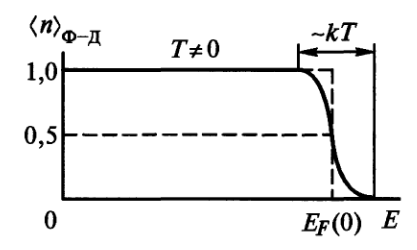
\includegraphics[width=.8\linewidth]{img/write-05/fermi-dirak-T-notzero}
	\caption{Распределение Ферми-Дирака при $T\neq 0$}
	\label{fig:fermi-dirak-t-notzero}
\end{wrapfigure}

Химический потенциал $\mu$, очевидно, имеет размерность энергии, а в случае фермионов называется \textit{энергией Ферми} или \textit{уровнем Ферми}, обозначается $E_F$.

Анализируя выражение $<n>_{\textsc{Ф-Д}}$ получим, что
\begin{align}
	T=0: <n>_{\textsc{Ф-Д}} = \begin{cases}
		1, E<E_F(0),\\
		0, E>E_F(0),
	\end{cases}
\end{align}
то есть при $T=0$ распределение принимает вид ступеньки единичной высоты, обрывающейся при $E=E_F(0)$. При $T\neq 0$ см. Рис \ref{fig:fermi-dirak-t-notzero}.
 \newpage
  \subsection{Сформулировать, какие частицы называются бозонами, привести примеры Бозе-частиц.
Сформулировать правило заполнения состояний Бозе- частицами. Используя формулу Больцмана
для энтропии, вывести распределение Бозе-Эйнштейна}


 \newpage
  \subsection{Описать явление термоэлектронной эмиссии. Рассматривая металл как потенциальный
ящик конечной глубины, заполненный «свободными» электронами, вывести формулу для плотности
тока насыщения $J_s$ термоэлектронной эмиссии.}

Термоэлектронная эмиссия -- излучение/испускание электронов из твердого тела при его нагреве.

Объектом исследования будет некий катод в вакууме, который кроме всего прочего мы нагреваем,
а вокруг него на некотором расстроянии находится анод -- в простом случае просто проводящая
пластина, с которой мы снимаем ток. Если рассматривать металл как потенциальный ящик конечной
глубины, получаем, что высота потенциального барьера $U_0$ вляется т.н. <<работой выхода>>
металла.

Током насыщения просто называется ток на аноде (на самом деле в более общем случае между 
катодом и анодом ещё приложено некоторое напряжение, и в том случае током насыщения называется
именно максимальное значение тока при разных напряжениях).

Плотность тока насыщения: $\vec{J} = q n \vec{v}$, где $\vec{v}$ -- дрейфовая скорость, 
$n$ -- концентрация зарядов, $q$ -- заряд частицы. Ясно, что электроны некоторым образом
распределены по скоростям, а в этой формуле нас интересуют только энергии
$E > U_0 = E_F + A_B$. Соотвественно этому, $d J_x = e v_x dn_e (v_x)$, а
$dn_{e, [E, E+\Delta E]} \sim \dfrac{\sqrt{E}}{e^{\dfrac{E-E_F}{kT}} + 1} dE$ -- см.
распределение свободных электронов. Для свободных электронов: $E = \dfrac{p^2}{2m}$,
следовательно,
\[
  \sqrt{E} \sim p, dE \sim p dp \Rightarrow \sqrt{E} dE \sim p^2 dp \sim 4\pi p^2 p^2 dp = d \Omega_p,
\]
где $d\Omega_p$ -- объём в фазовом пространстве $\vec{p} (p_x, p_y, p_z)$. Тогда
\[
  dn_{e, [p, p+\Delta p]} \sim \dfrac{d\Omega_p}{e^\dfrac{E(p) - E_F}{kT} + 1}
  \Rightarrow
  dn_e (\vec{p}) = \dfrac{dp_x dp_y dp_z}{e^\dfrac{E(p) - E_F}{kT} + 1}
\]
так как $v \sim p$, $\vec{v}$ сонаправлен с $\vec{p}$ и $dn_e (v_x) \sim dn_e(p_x)$.
Учитывая также, что $E > U_0 = E_F + A_B, A_B \gg kT$, можно получить, что 
\[
  e^{\dfrac{E-E_F}{kT}} \gg 1
  \Rightarrow
  dn_e (\vec{p}) \sim e^{\dfrac{E_F}{kT}} \cdot e^{\dfrac{- E(\vec{p})}{kT}} dp_x dp_y dp_z
\]
Дальше что-то очень простое:
\[
  E(\vec{p}) = E(p) = \dfrac{p_x^2 + p_y^2 + p_z^2}{2m_e}.
\]
Из этого найдём распределение $dn_e (p_x)$:
\[
  dn_e (p_x) = \int_\Omega dn_e (\vec{p}) = e^{\dfrac{E_F}{kT}} \cdot 
  e^{- \dfrac{p_x^2}{2m_e kT}} dp_x \cdot 
  \int_\mathbb{R} e^{- \dfrac{p_y^2}{2m_e kT}} dp_y \cdot 
  \int_\mathbb{R} e^{- \dfrac{p_z^2}{2m_e kT}} dp_z
  \sim T e^{\dfrac{E_F}{kT}} \cdot e^{-\dfrac{p_x^2}{2m_e kT}} dp_x
\]
Объединяя все полученные результаты:
\begin{multline*}
  dJ_x \sim v_x \cdot dn_e (v_x) \sim p_x dn_e (p_x)
  \Rightarrow
  dJ_x \sim P_x T e^{\dfrac{E_F}{kT}} \cdot e^{-\dfrac{p_x^2}{2m_e kT}} dp_x
  \Rightarrow \\
  \Rightarrow
  J_x \sim T e^{\dfrac{E_F}{kT}} \int_{p_x, \min}^{+\infty} e^{-\dfrac{p_x^2}{2m_e kT}} p_x dp_x
  \sim T^2 e^{\dfrac{E_F}{kT}} \cdot e^{-\dfrac{(E_F + A_B)}{kT}}
  = T^2 e^{- \dfrac{A_B}{kT}}
\end{multline*}
здесь не очевидно было что такое $p_{x, \min}$, а это такой импульс, что энергия такой частицы
равна $U_0$, то есть $\dfrac{p_{x, \min}^2}{2m_e} = U_0$.
 \newpage
  \subsection{Описать явление «холодной» эмиссии. Рассматривая металл как потенциальный ящик
конечной глубины заполненный «свободными» электронами, получить зависимость для плотности
тока $J$ «холодной» эмиссии от напряженности приложенного поля. Объяснить, почему холодная
эмиссия не может быть объяснена классической физикой}
Холодная эмиссия -- излучение/испускание электронов из твердого тела за счет туннельного
эффекта. Аналогично термоэлектронной эмиссии, есть катод, с которого будут вылетать электроны,
он погружён в вакуум, над поверхностью катода пластина -- анод, которая ловит электроны и мы 
смотрим ток, создаваемый ими (см. раздел \ref{sec:o244}).
Потенциальная энергия в зависимости от $x$ -- расстояния от поверхности
металла: 
$U(x) = U_0 - e \varepsilon x$, $x>0$.
Мы опустили слагаемое $ (ke^2)/(4x) $ из раздела \ref{sec:o244}, поскольку как
видно из графика в том же разделе, даже при небольших значениях $ x $ оно мало
влияет на общее значение потенциальной энергии (вследствие малости $ ke^2 $).
\begin{figure}[H]
  \centering
  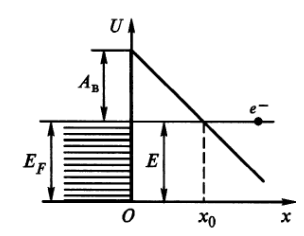
\includegraphics[width=.4\linewidth]{img/write-08/barier.png}
  \caption{Вид потенциала при холодной эмиссии}
  \label{fig:cold-emission}
\end{figure}

Вероятность туннелирования электрона определяется
коэффициентом прохождения $D$ через потенциальный барьер:
\[
  J_{\varepsilon} \sim D = \exp \left\{ - \dfrac{2}{\hbar} \int_0^{x_0} \sqrt{2m_e (U(x) - E)} \, dx \right\},
\]
где $x_0$ удовлетворяет уравнению
$U(x_0) = E_F \Leftrightarrow x_0 = \dfrac{U_0 - E_F}{e \varepsilon}$.
Преобразуем интеграл
\[
  - \dfrac{2}{\hbar} \int_0^{x_0} \sqrt{2m_e (U(x) - E)} \, dx 
  = - \dfrac{2}{\hbar} \sqrt{2m_e e \varepsilon} \int_0^{x_0} \sqrt{ x_0 - x } \, dx
  = - \dfrac{4}{3} \dfrac{2m_e}{e\hbar} (E_F + A_B - E)^{3/2} \dfrac{1}{\varepsilon}
  = - \dfrac{\varepsilon_0}{\varepsilon},
\]
то есть $J_x \sim e^{- \dfrac{\varepsilon_0}{\varepsilon}}$. На практике получаются очень
маленькие числа, так как $\varepsilon_0 \sim 10^{-8} \dfrac{\text{B}}{\text{м}}$.
 \newpage
  \subsection{Трансляционная симметрия твердых тел. Оператор трансляции и его собственные значения.
Сформулировать теорему Блоха (F. Bloch). Модель Кронига-Пени (R. Kronig, W. Penney) и ее
решение. Показать, что полученный спектр энергий представляет собой совокупность зон.
Заполнение зон в металлах, полупроводниках и диэлектриках}

см. Алексеев экзамен \#2


 \newpage
  \subsection{Электропроводность $\sigma$ чистых полупроводников. Подвижность $\mu$ носителей заряда.
Эффективная масса $m^*$. Вывести формулы для концентрации $n_e$ электронов и дырок $n_h$
в чистых полупроводниках. Найти положение уровня Ферми в чистых полупроводниках при $T=0$.
Температурная зависимость собственной проводимости полупроводников.}

\paragraph{Эффективная масса} рассмотрим группу электронов полуклассически: $p = \hbar k$, тогда
групповая скорость:
\[
  v_\text{гр} = \dfrac{\partial \omega}{\partial k} = \dfrac{\partial E}{\partial p} 
  = \dfrac{\partial E}{\partial k} \left( \dfrac{\partial p}{\partial k}  \right)^{-1}
  = \dfrac{1}{\hbar} \dfrac{\partial E}{\partial k} 
\]
в полуклассическом рассмотрении: <<$\vec{F} = \dfrac{\partial \vec{p}}{\partial t},
\vec{a} = \dfrac{\partial \vec{v}}{\partial t}$>>. Тогда:
\[
  \dfrac{\partial v_\text{гр}}{\partial t}
  = \dfrac{1}{\hbar} \dfrac{\partial }{\partial t} \left( \dfrac{\partial E}{\partial k} \right)
  = \dfrac{1}{\hbar} \dfrac{\partial }{\partial k} \left( \dfrac{\partial E}{\partial k}  \right) \cdot \dfrac{\partial k}{\partial t} 
  = \dfrac{1}{\hbar^2} \dfrac{\partial^2 E}{\partial k^2} \cdot \dfrac{\partial p}{\partial t}
  = a 
\]
сопоставляя определение силы и это выражение, получаем, что эффективная масса $m^* = \hbar^2 / \dfrac{\partial^2 E}{\partial k^2}$. Такая масса учитывает, что электрон/дырка
находятся в периодическом кристалле.

\paragraph{Электропроводность твердых тел} $\vec{J} = en \vec{v}_d$, $\vec{v}_d = \vec{a} \cdot \tau$, где $\tau$ -- время <<релаксации>> между соударениями с рассеивающими элементами. Тогда:
\begin{equation}\label{write:10:v_d}
  \vec{a} = \dfrac{\vec{F}}{m^*} = \dfrac{e\vec{E}}{m^*}
  \Rightarrow
  \vec{J} = \dfrac{e^2 \tau}{m^*} n \vec{E}
  \Rightarrow
  \vec{v}_d = \dfrac{e \tau}{m^*} \vec{E} = \mu \vec{E}
\end{equation}
$\mu$ называют подвижностью. $\vec{J} = \dfrac{1}{\rho_0} \vec{E} = \sigma \vec{E}$ -- $\rho$ --
удельное сопротивление, $\sigma$ -- удельная проводимость.

\paragraph{Концентрация электронов и дырок} концентрация свободных электронов:
\[
  dn_e = f_\text{ФД} (E) dN_e = f_\text{ФД} g(E) dE, g(E) \sim \sqrt{E}.
\]
Сдвинем энергии так, чтобы 0 энергии приходился на верхнюю часть зоны валентности. 
Нас интересуют только электроны, находящиеся в зоне проводимости, то есть энергия которых
больше ширины запрещённой зоны $E_g$. Концентрацию электронов можно найти путём интегрирования:
$n_e = \int dn_e$, однако, используем также то, что $E-E_F \gg kT$, тогда в знаменателе у
распределения Ф-Д можно пренебречь единицей. Тогда:
\[
  n_e \sim \int_{E_g}^{+\infty} \sqrt{E-E_g} e^{-\dfrac{E}{kT}} dE \sim \dots
  \sim (m_e^*)^{3/2} T^{3/2} \cdot e^{\dfrac{E_F - E_g}{kT}}
\]
У дырок наоборот, рассматривается только энергии меньше нуля, для них так же верно
$E<0 \Rightarrow |E-E_F| \gg kT$, тогда
$1 - f_\text{ФД} = 1 - \dfrac{1}{e^{\dots} + 1} \approx 1 - \left( 1 - e^{\dots} \right) = e^{\dfrac{E-E_F}{kT}} $. 
\[
  n_h \sim \int_{-\infty}^0 \sqrt{-E} \cdot e^{\dfrac{E}{kT}} dE \sim (m_h^*)^{3/2} T^{3/2} e^{-\dfrac{E_f}{kT}}
\]

\paragraph{Положение уровня Ферми в чистых полупроводниках}

Когда полупроводник чистый, концентрация электронов в зоне проводимости равна концентрации электронов в зоне валентности:
\[
  n_e = n_h \Leftrightarrow (m_e^*)^{3/2} T^{3/2} e^{\dfrac{E_G - E_g}{kT}} = (m_h^*)^{3/2} T^{3/2} e^{-\dfrac{E_F}{kT}} 
  \Leftrightarrow
  E_F(T) = \dfrac{3}{4} kT \ln (\dfrac{m_h^*}{m_e^*}) + \dfrac{E_g}{2}
\]
при $T = 0$, соотвественно, уровень Ферми находится ровно по середине запрещённой зоны.

\paragraph{Температурная зависимость}
\[
  \sigma = e^2 \left( \dfrac{n_e \tau_e}{m_e^*} + \dfrac{n_h \tau_h}{m_h^*} \right) 
\]
при изменении температуры качественно меняется только время релаксации. Оценим его из классических соображений. Рассмотрим цилиндр небольшого радиуса, который окружает траекторию рассматриваемого электрона. Электрон движется с некоторой усредненной скоростью $<v>$, поэтому рассмотрим цилиндр длиной $<v> \delta t$. Количество столкновений $N$ с рассеивающими частицами пропорционально количеству частиц в этом цилиндре, а оно в свою очередь пропорционально концентрации рассеивающих частиц. Среднее время между столкновениями: $\tau = \dfrac{t}{N} \sim \dfrac{1}{n <v>}$. Рассеиваются наши электроны на фононах, которые являются бозонами, поэтому концентрация подчиняется статистике Б-Э. Поэтому:
\[
  \tau \sim \dfrac{1}{n_\text{Ф} <v>} \sim \dfrac{e^{\dfrac{E_0}{kT}} - 1}{v}
  \sim \dfrac{1}{T^{1/2} T} \sim T^{-3/2}
\]
а проводимость в таком случае:
\[
  \sigma \sim n_e \tau \sim T^{3/2} e^{-E_g / (kT)} T^{-3/2} \sim e^{-E_g / (kT)}
\]
 \newpage

  \newpage

  \section{Устная часть}
  \subsection{Фундаментальные понятия и принципы Квантовой Механики}

\subsubsection{Волны Де Бройля}

\begin{multicols}{2}
	
\paragraph{Общий случай} Плоская волна частотой $\omega$, распространяющаяся вдоль оси $x$:
\begin{equation*}
	\xi(x,t) = A \exp \left\{-i(\omega t -kx)\right\},
\end{equation*}
где $A$ - амплитуда, $k=\frac{2\pi}{\lambda}$ - волновое число.

\paragraph{Гипотеза Де Бройля} 
\thispagestyle{empty}
Свободной частице с энергией $E$ и импульсом $p$, движущейся вдоль $x$, соответсвует плоская волна:
\begin{equation*}
	\Psi(x, t) = A \exp \left\{-\frac{i}{\hbar}(E t - px)\right\}
\end{equation*}
Посмотрев на выражения волновых процессов в общем виде $\xi$ и для волны Де Бройля $\Psi$, заметим некоторые соотношения:
\begin{itemize}
	\item частота $\omega = \frac{E}{\hbar}$
	\item длина волны Де Бройля $\lambda_{\text{Б}}=\frac{2\pi\hbar}{p}$
	\item энергия $E = \hbar \omega = h\nu$
	\item $\vec p = \hbar \vec k$, где $\vec k$ - волновой вектор
\end{itemize}

\paragraph{Свойства волн Де Бройля}
\begin{enumerate}[label=\textbf{№~\arabic{enumi}}]
	\item В процессе распространения волны могут отражаться, преломляться, интерферировать и дифрагировать по обычным волновым законам
	
	\item Фазовая скорость $v_\text{фаз}$ - скорость, с которой распространяются точки волны с постоянной фазой.
	Выражение для фазовой скорости вытекает из условия постоянности фазы при его дифференцировании:
	\begin{equation*}
		Et-px=\mathrm{const} \overset{\dfrac{d}{dt}}{\longrightarrow} v_\text{фаз} = \frac{dx}{dt} = \frac{E}{p}.
	\end{equation*}
	При подстановке известных соотношений, а именно $E=mc^2$ и $p=mv$ в $v_\text{фаз}$, получим
	\begin{equation*}
		v_\text{фаз} = \frac{c^2}{v}
	\end{equation*} выражение для фазовой скорости\footnote{$v<c \implies v_\text{фаз} = \frac{c^2}{v} > c$ --- это не противоречит СТО. Ограничения, накладываемые СТО касаются скорости переноса массы/энергии, но фазовая скорость волны ничего из этого не характеризует.}.
	
	\item Групповая скорость $v_\text{гр}$
	\begin{equation*}
		v_\text{гр} = \frac{dw}{dk} = \frac{d(\hbar\omega)}{d(\hbar k)} = \frac{dE}{dp}
	\end{equation*}
	Возьмем известное всем выражение из теории относительности:
	\begin{equation*}
		E^2=p^2c^2+E_0^2=\left[E_0=m_0c^2\right]=E^2=p^2c^2+m_0^2c^4
	\end{equation*}
	Продифференцируем по t:
	\begin{equation*}
		2EdE=2pc^2dp\longrightarrow\frac{dE}{dp}=\frac{pc^2}{E}
	\end{equation*}
	Воспользовавшись этим знанием, получаем, что групповая скорость волны равна скорости движения частицы:
	\begin{equation*}
		v_\text{гр} = \frac{pc^2}{E} = \frac{pc^2}{mc^2} = \frac{p}{m} = v
	\end{equation*}
	
	\item Длина волны Де Бройля для нерелятивистских $(v\ll c)$ и релятивистких ($v\approx c$) частиц.
	\begin{itemize}
		\item Нерелятивисткий случай $(v\ll c)$:
		\begin{equation*}
		E_k=\frac{mv^2}{2}=\frac{p^2}{2m_0}\implies p=\sqrt{2m_0E_k}
		\end{equation*}
		\begin{equation*}
		\lambda_\text{Б}=\frac{2\pi\hbar}{p}=\frac{2\pi\hbar}{\sqrt{2m_0E_k}}
		\end{equation*}
		\item Релятивистский случай $(v\approx c)$:
		\begin{equation*}
		p=\frac{1}{c}\sqrt{E_k(E_k+2m_0c^2)} \Leftrightarrow
		\end{equation*}
		\begin{equation*}
		\Leftrightarrow p=\sqrt{2m_0E_k}\sqrt{1+\frac{E_k}{2m_0c^2}}
		\end{equation*}
		\begin{equation*}
			\lambda_\text{Б}'=\frac{2\pi\hbar}{p}=\frac{2\pi\hbar}{\sqrt{2m_0E_k}\sqrt{1+\frac{E_k}{2m_0c^2}}}
		\end{equation*}
		В этом выражении можно выделить нерелятивистскую дебройлевскую длину волны $\lambda_\text{Б}$, тогда 
		\begin{equation*}
			\lambda_\text{Б}'=\frac{\lambda_\text{Б}}{\sqrt{1+\frac{E_k}{2m_0c^2}}}
		\end{equation*}
	\end{itemize}
\end{enumerate}

\end{multicols}
\subsubsection{Соотношения неопределенностей Гейзенберга}
\begin{multicols}{2}
	\paragraph{Смысл}
	Двойственная корпускулярно-волновая природа микрочастиц накладывает ограничения на точность определения значений физических величин, характеризующих состояние частицы. Причем эти ограничения никак не связаны с точностью измерений, достижимой в конкретном эксперименте, а имеют принципиальное значение.
	\paragraph{Выражения для неопределенностей}
	\begin{equation*}
		\begin{cases}
		\left.\begin{array}{lll}
			\Delta p_x \Delta x & \geq \dfrac{\hbar}{2} &  \\[10pt]
			\Delta p_y \Delta y & \geq \dfrac{\hbar}{2} &  \\[10pt]
			\Delta p_z \Delta z & \geq \dfrac{\hbar}{2} &  
		\end{array}\right] \text{иногда пишут $\hbar$} \\[1.5cm]
		\begin{array}{rr}
			\Delta E \Delta t  & \geq \hbar 
		\end{array}
		\end{cases},
	\end{equation*}где $\Delta P_{x}$ --- неопределенность импульса $P_{x}$, \\
	$\Delta x$ --- неопределенность координаты $x$,\\
	$\Delta E$ --- неопределенность энергии,\\
	$\Delta t$ (иногда пишут $\tau$) --- среднее \textit{время жизни} в данном энергетическом состоянии.
	
	\paragraph{Общий ход вывода соотношений для моментов и координат}
	\begin{figure}[H]
		\centering
		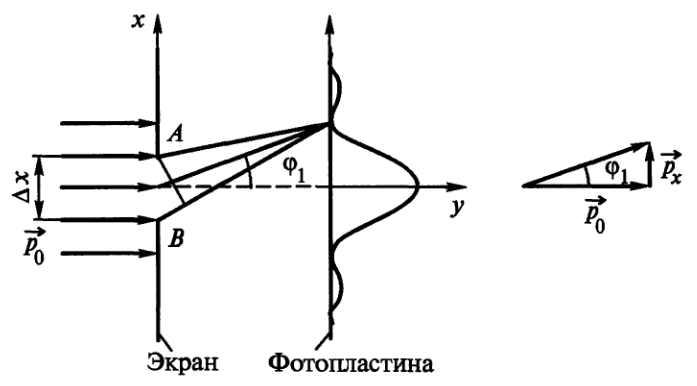
\includegraphics[width=.9\linewidth]{img/oral-01/electron-difraction}
		\caption{Картина дифракции электрона на щели}
		\label{fig:electron-difraction}
	\end{figure}
	(см Рис. \ref{fig:electron-difraction}) Пусть падающий электрон обладает импульсом $\vec p_0$. По гипотезе Де Бройля поставим в соответствие этому электрону плоскую волну с волновым вектором $\vec k = \frac{\vec p_0}{\hbar}$ и длиной волны $\lambda_{\text{Б}}=\frac{2\pi\hbar}{p_0}$.
	
	До прохождения щели известен импульс электрона $p_x=p_z=0,\, p_y=p_0$, а его координата $x$ неизвестна.
	
	При прохождении щели неопределенность координаты $x$ становится равной $\Delta x$, появляется неопределенность импульса $\Delta p_x$, обусловленная дифракцией электронов на щели\footnote{Электроны после прохождения щели описываются теперь не плоской, а расходящейся волной, интенсивность которой зависит от угла дифракции $\varphi$.}. Меняется также и проекция $p_x$ импульса электрона на ось $x$.
	
	Центральный дифракционный максимум, в который попадет большинство электронов, описывается углом $\varphi_1$, задающим первый минимум интенсивности. Из теории дифракции ($\Delta x \sin(\varphi_k)=k\lambda,\,k\in\mathbb{N}$) запишем уравнение для нахождения $\varphi_1,\,(k=1)$:
	\begin{equation*}
		\Delta x \sin \varphi_1=\lambda_{\text{Б}}
	\end{equation*}
	За счет малости $\varphi_1$ используем приближение:
	\begin{equation*}
		\frac{\lambda_{\text{Б}}}{\Delta x} = \sin \varphi_1 \approx \tg \varphi_1
	\end{equation*}
	В то же время угол $\varphi_1$ можно выразить через проекции $p_x,\,p_y$ импульса электрона:
	\begin{equation*}
		\tg \varphi_1 = \frac{p_x}{p_y} = \frac{p_x}{p_0}
	\end{equation*}
	Считая, что неопределенность $\Delta p_x$ сравнима с $p_x$, получаем:
	\begin{equation*}
		\tg \varphi_1 \approx \frac{\Delta p_x}{p_0}
	\end{equation*}
	Отсюда следует, что:
	\begin{equation*}
		\tg \varphi_1 \approx \frac{\Delta p_x}{p_0} \approx \frac{\lambda_{\text{Б}}}{\Delta x}
	\end{equation*}
	Окончательно получаем:
	\begin{equation*}
		\Delta x \Delta p_x \approx \lambda_{\text{Б}}p_0
	\end{equation*}
	Поскольку $\lambda_{\text{Б}}=\frac{2\pi\hbar}{p_0}$, то с учетом сделанных приближений и упрощений:
	\begin{equation*}
		\Delta x \Delta p_x \approx \underset{\text{пишут по разному}}{2\pi\hbar \geq \hbar \geq \frac{\hbar}{2}}
	\end{equation*}
	
	Поскольку ось $x$ физически ничем не была выделена, то аналогичное соотношение оказывается справедливым для других координатных осей $y$ и $z$.
\end{multicols}

\subsubsection{Постулаты квантовой механики}

\subsubsection{Принцип суперпозиции квантовых состояний}

\subsubsection{Принцип неразличимости тождественных частиц}
Состояние электрона в атоме определяется набором четырёх квантовых чисел:
\begin{table}[H]
	\begin{center}
		\begin{tabular}{c|r|l}
			1 &            главное & $n\in\mathbb{N}$                                \\[5pt]
			2 &        орбитальное & $l\in[0,n-1]$                                   \\[5pt]
			3 &          магнитное & $m\in[-l,l]$                                    \\[5pt]
			4 & магнитное спиновое & $m_s\in\left\{\frac{-1}{2},\frac{1}{2}\right\}$ \\[5pt]
		\end{tabular}
	\end{center}
	\caption{Квантовые числа}
\end{table}
\paragraph{Принцип неразличимости тождественных частиц} Тождественные частицы экспериментально различить невозможно.
\paragraph{Математическая запись}
\begin{equation*}
	\left|\Psi(x_1,x_2)\right|^2 = \left|\Psi(x_2,x_1)\right|^2,
\end{equation*}
где $x_1$ и $x_2$ --- соответственно совокупность пространственных и спиновых
координат первой и второй частиц. Возможны два случая:
\begin{table}[H]
	\begin{center}
	\begin{tabular}{|l|c|c|}
		\hline
		Случай   &         симметричный          &        антисимметричный        \\ \hline
		Запись   & $\Psi(x_1,x_2)=\Psi(x_2,x_1)$ & $-\Psi(x_1,x_2)=\Psi(x_2,x_1)$ \\ \hline
		Спин     &      $m_s\in\mathbb{Z}$       & $m_s\in\mathbb{Z}+\frac{1}{2}$ \\ \hline
		Название &         \text{бозоны}         &        \text{фермионы}         \\ \hline
		Примеры  &     $\pi$-мезоны, фотоны      &  электроны, протоны, нейтроны  \\ \hline
	\end{tabular}
	\end{center}
\end{table}
 \newpage
  \subsection{Следствия из основных положений}

\subsubsection{Уравнение непрерывности для плотности вероятности, как следствие основных
постулатов и уравнения Шрёдингера (вывод)}

Уравнение Шредингера:
\[
  -i \hbar \dfrac{\partial \Psi}{\partial t} = - \dfrac{\hbar^2}{2m} \nabla^2 \Psi + U \Psi,
\]
комплексно сопряженное уравнение:
\[
  -i \hbar \dfrac{\partial \Psi^*}{\partial t} = - \dfrac{\hbar^2}{2m} \nabla^2 \Psi^* + U \Psi^*,
\]

Умножим обычное на $\Psi^*$, а компескно сопряженное умножим на $\Psi$, потом сложим:
\[
  i \hbar \left( \Psi^* \dfrac{\partial \Psi}{\partial t} + \Psi \dfrac{\partial \Psi^*}{\partial t} \right)
  = - \dfrac{\hbar^2}{2m} \left( \Psi^* \nabla^2 \Psi - \Psi \nabla^2 \Psi^* \right) 
  \Rightarrow
  \left( \Psi^* \dfrac{\partial \Psi}{\partial t} + \Psi \dfrac{\partial \Psi^*}{\partial t} \right)
  = \dfrac{i \hbar}{2m} \left( \Psi^* \nabla^2 \Psi - \Psi \nabla^2 \Psi^* \right) 
\]
левая часть равенства представляет собой $\dfrac{\partial \Psi^* \Psi}{\partial t} =
\dfrac{\partial |\Psi|^2}{\partial t}$, то есть производную плотности вероятности $\rho_p$
по времени. В правой части преобразуем:
\[
  \left( \Psi^* \nabla^2 \Psi - \Psi \nabla^2 \Psi^* \right)
  = \nabla \left( \Psi^* \nabla \Psi - \Psi \nabla \Psi^* \right)
\]
(это выражение проверяется в лоб). Обозначая $ - \dfrac{i \hbar}{2m} \left( \Psi^* \nabla \Psi - \Psi \nabla \Psi^* \right) = \vec{J}_p$, окончательно получаем:
\[
  \dfrac{\partial \rho_p}{\partial t} = - \nabla \vec{J}_p =  - \operatorname{div} \vec{J}_p.
\]
Это выражение называется уравнением непрерывности для плотности вероятности.

\subsubsection{Симметричные и антисимметричные состояния}

Для системы нескольких частиц, волновая функция представляется в виде: $\Phi( \vec{q}_1, \vec{q}_2, \dots, \vec{q}_n )$. Рассмотрим оператор перестановки $\hat{P}_{ij}$:
\[
  \hat{P}_{ij} \Psi(\vec{q}_1, \dots, \vec{q}_i, \dots, \vec{q}_j, \dots, \vec{q}_n)
  = \Psi(\vec{q}_1, \dots, \vec{q}_j, \dots, \vec{q}_i, \dots, \vec{q}_n)
\]
рассмотрим спектр этого оператора:
\[
  \hat{P}_{ij} \Psi = \lambda \Psi, \hat{P}^2_{ij} \Psi = \Psi = \lambda^2 \Psi 
  \Rightarrow
  \lambda = \pm 1.
\]
Функции $\Psi$, у которых $\lambda = 1$, называются симметричными, а другие -- антисимметричными. Причём несложно доказать, что если системе одинаковых частиц в некоторый момент времени соответствовала функция (анти) симметричная, то и в последующие моменты времени она останется такой же:
\[
  - i \hbar \dfrac{\partial \Psi}{\partial t} = \bar{H} \Psi
\]
ну и вот справа будет функция такой же симметричности как и $\Psi$, поэтому и слева тоже.

\subsubsection{Принцип Паули в строгой формулировке}

В одном и том же квантовом состоянии может находится не более одного фермиона. Состояние можно
характеризовать 4 величинами $L_1, L_2, L_3, L_s$: все эти величины одновременно измеримы. Первые
3 величины относятся к движению центра масс и незваисимы друг от друга, $L_s$ описывает состояние
спина электрона. 

Пример такой совокупности величин: $E_{n, l} = L_1; L^2 = L_2, L_z = L_3; L_s = m_s$.

Тогда принцип Паули можно также переформулировать следующим образом: в процессе измерения над 
системой каждая четвёрка величин $L_1, L_2, L_3, L_4$ может быть получена не более одного раза.

\subsubsection{Нахождение среднего значения физической величины (вывод)}

Пусть некоторой физической величине $f$ соотвествует оператор $\hat{f}$. Найдём его собственные значения и обозначим их $f_n$, а собственные функции -- $\Psi_n$.

Тогда любое состояние $\Psi$ раскладывается по базису из собственных функций этого оператора:
\[
  \Psi = \sum_n c_n \Psi_n
\]
это утверждение носит название 3-его постулата КМ. Причём вероятность $P(f = f_n)$ равняется квадрату модуля коэффициента перед соотвествующей собственной функцией:
\[
  P(f = f_n) = P_n = c_n^* c_n.
\]

Тогда среднее значение (матожидание) некоторой величины $f$ выражается:
\begin{multline*}
  <f> = \sum_n P_n f_n
  = \sum_n c_n^* c_n f_n
  = \sum_n c_n^* f_n \int \Psi_n^* \Psi dV
  = \sum_n c_n^* \int \Psi \hat{f} \Psi_n^*
  = \int \Psi (\hat{f} \sum_n c_n \Psi_n)^* dV = \\
  = \int \Psi (\hat{f} \Psi)^* dV
  = \int \Psi^* (\hat{f} \Psi) dV
\end{multline*}

\subsubsection{Дискретность спектра энергий для связанных состояний квантовых систем
(Объяснить связь с основными постулатами)}

Связным состоянием называется такое состояние, в котором частица движется в ограниченной области
пространства $\Omega$, следовательно, граничное условие для $\Psi$:
$\left. \Psi \right|_{\partial \Omega} = 0$. В таком случае спектр энергий квантуется.

Из ландафщица:

Спектр собственных значений энергии может быть как дискретным, так и непрерывным.
Стационарное состояние дискретного спектра всегда соответствует финитному движению
системы, т. е. движению, при котором система или какая-либо ее часть не уходит на
бесконечность. Действительно, для собственных функций дискретного спектра интеграл
$\int |\Phi|^2 dq$, взятый по всему пространству, конечен. Это, во всяком случае,
означает, что квадрат $|\Phi|^2$ достаточно быстро убывает, обращаясь на бесконечности в
нуль. Другими словами, вероятность бесконечных значений координат равна нулю, т. е.
система совершает финитное движение или, как говорят, находится в связанном состоянии.

Для волновых функций непрерывного спектра интеграл $\int | \Phi |^2 dq$ расходится.
Квадрат волновой функции $|\Phi|^2$ не определяет здесь непосредственно вероятности
различных значений координат и должен рассматриваться лишь как величина, пропорциональная
этой вероятности. Расходимость интеграла $\int | \Phi |^2 dq$ всегда бывает связана с тем,
что $|\Phi|^2$ не обращается на бесконечности в нуль (или обращается в нуль недостаточно
быстро). Поэтому можно утверждать, что интеграл $\int | \Phi |^2 dq$, взятый по
области пространства, внешней по отношению к любой сколь угодно большой, но конечной
замкнутой поверхности, будет все же расходиться. Это значит, что в рассматриваемом
состоянии система (или какая-либо ее часть) находится на бесконечности. Для волновой функции,
представляющей собой суперпозицию волновых функций различных стационарных состояний
непрерывного спектра, интеграл $\int |\Phi|^2 dq$ может оказаться сходящимся, так что
система находится в конечной области пространства. Однако с течением времени эта область
будет неограниченно смещаться, и в конце концов система уходит на бесконечность.


\subsubsection{Квантовое туннелирование и его проявление в различных явлениях ($\alpha$-распад, холодная эмиссия, тунельный микроскоп)}

Определение. Туннельный эффект или туннелирование - это явление преодоления микрочастицей
потенциального барьера в случае, когда её полная энергия (остающаяся при туннелировании
неизменной) меньше высоты барьера.

\paragraph{Альфа распад}
Альфа-частица испытывает туннельный переход через потенциальный барьер, обусловленный
ядерными силами, поэтому альфа-распад является существенно квантовым процессом.

\paragraph{Холодная эмиссия}


\paragraph{Тунельный микроскоп}
Рассматривать отдельные атомы можно с помощью устройства, использующего квантовый эффект
туннелирования – сканирующий туннельный микро- скоп (СТМ). Точнее, сканирующий туннельный
микроскоп не рассматривает, а как бы «ощупывает» ис- следуемую поверхность. Очень тонкая
игла-зонд с острием толщиной в один атом перемещается над поверхностью объекта на расстоянии
порядка одного нанометра. При этом согласно законам квантовой механики, электроны преодолевают
вакуумный барьер между объектом и иглой – туннелируют, и между зондом и образцом начинает
течь ток. Сила этого тока очень сильно зависит от расстояния между концом иглы и поверхностью
образца – при изменении зазора на десятые доли нанометра сила тока может возрасти или
уменьшиться на порядок. Так что, перемещая зонд вдоль поверхности с помощью пьезоэлементов
и отслеживая изменение силы тока, можно исследовать ее рельеф практически «на ощупь».

 \newpage
  \subsection{Элементы статистической физики}
\subsubsection{Принцип детального равновесия и его применение (вывод закона Кирхгофа, связь $r_{T, \omega}^*$ vs $u_{T, \omega}$, формула Эйнштейна для коэффициентов A и B)}
\paragraph{Принцип детального равновесия.}\label{sec:teplo} В нагретых телах часть внутренней
энергии вещества может превращаться в энергию излучения. Эксперименты
показывают, что тепловое излучение имеет непрерывный спектр. Распределение
энергии излучения по спектру зависит от температуры (позже выясняется, что
максимум смещается к низким частотам с увеличением температуры, хотя общая
энергия возрастает). 

Если несколько тел окружить полостью с идеально отражающими непроницаемыми
стенками, то со временем установится \emph{тепловое равновесие}, причём оно
будет устойчивым. Зеркальные стенки можно заменить стенками из одинакового
материала с поддерживаемой температурой. В других видах излучения равновесия
быть не может.

Равновесное тепловое излучение однородно, то есть его плотность
энергии одинакова во всех точках внутри полости, где оно 
заключено. Такое излучение изотропно, однородно и неполяризованно --- оно 
содержит все возможные направления распространения и 
направления колебаний векторов $ \mathbf E $ и $ \mathbf H $.

В опыте с равновесным излучением, конечно, каждое тело будет излучать в единицу
времени столько же энергии частоты $ \omega_0 $, сколько поглощать. Это и есть
\emph{принцип детального равновесия}. Тогда отношение испускательной способности
к поглощательной одинаково для всех тел в природе и является функцией частоты и
температуры. 
\[
  \left( \frac{r_{\omega, T}}{a_{\omega, T}} \right)_1 = \left( \frac{r_{\omega,
  T}}{a_{\omega, T}} \right)_2 = \ldots = \frac{r^\ast_{\omega, T}}{1} =:
  f(\omega, T).
\]
Аналогичная цепочка равенств, конечно, справедлива и для длин волн. Это и есть
\emph{закон Кирхгофа}. Он может быть получен и другим опытом, где на АЧТ
маленький кусок поверхности $ d\sigma $ заменяется обычным непрозрачным телом. Этот кусок
поглащает $ a_{\omega, T} $-ую часть, а отражает $ 1 - a_{\omega, T} $. Падает на него по-прежнему $
r^\ast_{\omega, T}d\sigma $ энергии. Поглащает он $ a_{\omega, T}
r^\ast_{\omega, T} d\sigma $, а испускает $ r_{\omega, T} d\sigma $. Снова
приходим к закону Кирхгофа. Заметим, что этот подменённый кусок $ d\sigma $ для
внутреннего наблюдателя ничем не будет отражаться от остальных, поскольку
недоиспущенную энергию он будет отражать: 
\[
  d\sigma [r_{\omega, T} + (1- a_{\omega, T}) r^\ast_{\omega, T}] =
  r^\ast_{\omega, T} d\sigma.
\]

Рассмотрим куб с ребром $ l $ и зеркальными стенками. Поместим внутрь малое по
размеру АЧТ с температурой $ T $. Разложим объёмную плотность энергии  
\[
    u(T) := \frac{dW}{dV}
\]
по частотам: 
\[
  u_{\omega, T} := \frac{dW_{\omega, \omega + d\omega}}{dVd\omega}.
\]
Рассмотрим излучение вблизи элементарной площадки $ \Delta S $ этого АЧТ.

\begin{figure}[h!]
  \centering
  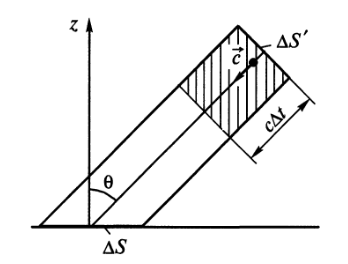
\includegraphics[width=0.4\textwidth]{img/oral-03/acht.png}
  \label{fig:acht}
\end{figure}

Плотность вблизи этой площадки равномерно распределена по всевозможным
направлениям телесного угла $ 4\pi $. Поэтому плотность энергии излучения,
приходящегося на телесный угол $ d\Omega = \sin \theta d\theta d\varphi $, то
есть падающего на площадку под углом $ \theta $ к её нормали (?), можно записать в
виде
\[
    d\tilde u = u(T) \frac{d\Omega}{4\pi}.
\]
Тогда за время $ \Delta t $ на эту площадку попадёт вся энергия излучения,
заключенная в заштрихованном объёме, то есть 
\[
    dw = d\tilde u c \Delta t \Delta S' = d\tilde u c\Delta t \Delta S \cos
    \theta = \frac{c}{4\pi} u(T)\cos \theta \sin\theta d\theta d\varphi\Delta S
    \Delta t.
\]
Найдём полный поток энергии $ \Phi $ излучения, падающего на единицу поверхности
в единицу времени: 
\[
    \Phi = \frac{c}{4\pi}u(T) \int\limits_{0}^{2\pi}d\varphi
    \int\limits_{0}^{\pi/2}\cos\theta\cdot \sin\theta\,d\theta =
    \frac{c}{4}u(T).
\]
В условиях равновесия, конечно, $ \Phi = R^\ast $. Причём данная формула
справедлива и для спектральных характеристик: 
\[
  r^\ast_{\omega, T} = \frac{c}{4}u_{\omega, T}.
\]


\paragraph{Формула Эйнштейна для коэффициентов A и B.} см. письменный вопрос \ref{einstein-a-b}

\subsubsection{Плотность квантовых состояний}
Найдём число квантовых состояний, по которым могут распределяться частицы, при
условии, что энергия этих состояний не превышает некоторого значения $ E $.
Пусть сначала частица находится в трёхмерной потенциальной яме с непроницаемыми
стенками. Энергия в такой яме равна 
\[
  E = \frac{\pi^2\hbar^2}{2m_0} \left[ \left( \frac{n_1}{a_1} \right)^2 + \left(
  \frac{n_2}{a_2}\right)^2 + \left( \frac{n_3}{a_3} \right)^2   \right],
\]
где $ a_1 $, $ a_2 $ и $ a_3 $ --- стороны прямоугольного параллелепипеда, а $
n_1 $, $ n_2 $, $ n_3 = 1, 2, 3,\ldots$ --- квантовые числа. Пусть $ E $ столь
велико, что спектр можно считать практически непрерывным.

В дискретном трёхмерном пространстве квантовых чисел введём обозначение  
\[
  r^2 = \frac{(n_1a_2a_3)^2 + (n_2a_1a_3)^2 + (n_3a_1a_2)^2}{(a_1a_2a_3)^{4/3}}
\]
и перепишем выражение для энергии в виде 
\[
  E = \frac{\pi^2\hbar^2}{2m_0(a_1a_2a_3)^{2/3}}r^2,
\]
откуда 
\[
  r = \frac{(a_1a_2a_3)^{1/3}\sqrt{2m_0E}}{\pi\hbar}.
\]

Теперь коль скоро $ n_1^2 + n_2^2 + n_3^2 < r^2 $, то и $ E < E_{\max} $ (?). Рассмотрев теперь сферу (её восьмую часть) с радиусом $ r $, найдём число
возможных состояний как объём этой фигуры:
\[
  G = \frac{1}{6}\pi r^3 J_z = \frac{1}{6} \pi \frac{ \left( \sqrt{2m_0E}
  \right)^3 }{\pi^3\hbar^3}J_z a_1a_2a_3,
\]
где $ J_z $ есть количество возможных проекций спина частицы (для электрона,
например, они принимают значения $ \pm 1/2 $, откуда $ J_z = 2 $).
Действительно, каждой точке пространства соответствует $ J_z $ состояний.
Поскольку $ a_1a_2a_3 $ представляет собой объём потенциальной ямы $ V $, а $
\sqrt{2m_0E} $ есть нерелятивистский импульс частицы $ p $, то соотношение можно
переписать в виде 
\[
  G = \frac{4}{3} \pi p^3 V \frac{J_z}{(2\pi\hbar)^3}.
\]
При этом $ (4\pi p^3)/3 $ есть не что иное, как объём шара радиусом $ p $
--- импульса, соответствущего максимальной энергии $ E $ --- в пространстве
импульсов $ p_x $, $ p_y $, $ p_z $. Таким образом, выражение для $ G $ в
фазовом пространстве $ x $, $ y $, $ z $, $ p_x $, $ p_y $, $ p_z $ имеет вид 
\[
  G = \frac{V_{\text{фаз}}}{(2\pi \hbar)^3} J_z,
\]
то есть $ G $ пропорционально фазовому объёму.

Оказывается, что данный результат справедлив для ям произвольной формы.

Таким образом, объём фазового пространства, приходящийся на одно квантовое
состояние, равен $ (2\pi\hbar)^3 = h^3 $. Запишем это следующим образом: 
\[
  \Delta x \Delta y \Delta z \Delta p_x \Delta p_y \Delta p_z = h^3,
\]
где $ \Delta x, \ldots \Delta p_x, \ldots $ --- размеры ячейки в фазовом пространстве, приходящейся
на одно состояние. При этом благодаря равноправности координат (?), например, $
\Delta x \Delta
p_x = 2\pi \hbar$. Этот результат, как легко видеть, согласуется с принципом 
неопределенности. Действительно, размеры ячейки фазового 
пространства, приходящейся на одно состояние, должны определяться
теми ограничениями на значения координаты и импульса, которые
накладывают соотношения неопределенностей.

Найдём теперь \emph{плотность квантовых состояний} $ g(E) $, то есть число
состояний, приходящихся на единичный интервал энергий. Найдём его, переписав в
виде 
\[
  g(E)  = \frac{dG}{dp} \frac{dp}{dE} = J_z \frac{dp}{dE} \frac{d}{dp} \left(
  \frac{4}{3} \frac{\pi p^3 V}{(2\pi \hbar)^3}\right) = J_z \frac{4\pi p^2
  V}{(2\pi\hbar)^3} \frac{dp}{dE}.
\]
Данное выражение является общим, то есть справедливым для любых частиц.

\subsubsection{Плотность мод колебаний электромагнитного поля в полости}
\label{sec:plot-mod}
\paragraph{Частотная.}
\emph{Модами}, или \emph{собственными колебаниями} называют набор характерных
для колебательной системы типов гармонических колебаний. 

Будем считать, что стенки либо зеркальные, либо однородные с поддерживаемой
температурой $ T $. В такой модели тепловое излучение может существовать только
в виде суперпозиции прямых и отражённых волн, то есть в виде \emph{стоячих
волн}, имеющих узлы на стенках полости. Направим $ \mathbf e_x $, $ \mathbf e_y
$, $ \mathbf e_z $ вдоль рёбер куба. Тогда для волны, распространяющейся строго
вдоль оси $ x $, условие образования стояей волны имеет вид 
\[
    l = n_1 \frac{\lambda}{2}, \quad n_1 = 1, 2, 3, \ldots,
\]
то есть на длине $ l $ между отражающими стенками должно укладываться целое
число длин полуволн. Так как для такой волны волновой вектор $ \mathbf k = k_x
\mathbf e_x $, где $ k_x = 2\pi/\lambda $. Аналогичные рассуждения для волн в
целом приводят к соотношениям  
\[
    k_x = n_1 \frac{\pi}{l}, \quad k_y = n_2 \frac{\pi}{l}, \quad k_z = n_3
    \frac{\pi}{l}.
\]
Здесь $ n_k $ могут уже принимать и нулевые значения, но не все разом. Тогда  
\[
  k = \frac{2\pi}{\lambda} = \frac{\omega}{c} = \frac{\pi}{l} \sqrt{n_1^2 + n_2^2 + n_3^2}.
\]
Каждой тройке $ n_1 $, $ n_2 $, $ n_3 $ соответствует одна стоячая волна.
Определим число стоячих волн, частоты которых не превышают $ \omega $.
Рассмотрим дискретное трёхмерное пространство квантовых чисел и сферу в нём
радиуса $ R = (\omega l)/(\pi c) $. Определим искомое число как восьмую часть
объёма этой сферы. Тогда  
\[
    \tilde N = \frac{1}{8} \frac{4}{3} \pi R^3 = \frac{1}{6}
    \frac{\omega^3l^3}{\pi^2 c^3} = \frac{1}{6} \frac{\omega^3}{\pi^2 c^3} V.
\]
Здесь $ V = l^3 $ --- объём полости, в которой заключено рассматриваемое
равновесное тепловое излучение.

Следует учесть, что электромагнитные волны --- поперечные
волны и в каждом направлении $ \mathbf k $ в полости в общем случае могут
распространяться две волны, поляризованные во взаимно 
перпендикулярных плоскостях. Поэтому число стоячих волн с частотой,
не превышающей заданного значения $ \omega $, следует определить как 
\begin{align}
  N &= 2\tilde N = \frac{1}{3} \frac{\omega^3}{\pi^2 c^3}V,\\
  dN &= \frac{\omega^2 d\omega}{\pi^2 c^3}V.
  \label{eq:mods}
\end{align}
Обозначим как $ \langle \varepsilon_\omega \rangle $ среднюю энергию стоячей
электромагнитной волны частоты $ \omega $, тогда при равновесии
\[
  u_{\omega, T}d\omega = \frac{dN\langle \varepsilon_\omega \rangle}{V},  
\]
откуда  
\[
  u_{\omega, T} = \frac{\omega_2}{\pi^2 c^3} \langle \varepsilon_\omega \rangle
= \frac{\hbar \omega^3}{\pi^2 c^3} \frac{1}{\exp(\frac{\hbar\omega}{kT}) - 1},
\]
где в последнем равенстве была использована формула Планка.

\paragraph{Энергетическая.}
Будем считать, что речь об электронах в полупроводнике. По определению энергетическая плотность состояний $ g(E) = dN/dE $, где $ dN $ ---
число состояний с энергией от $ E $ до $ E + dE $. Представим это число в виде $
dN = g(k)dV_k $, где $ g(k) $ --- плотность состояний в пространстве $ (k_x,
k_y, k_z) $ волновых векторов, а $ dV_k $ --- такой элемент объёма этого
пространства, в котором энергия изменяется от $ E $ до $ E + dE $.

Найдём сначала $ g(k) $. Пусть $ d\tau_k = dk_x dk_y dk_z $, а $ V_l = l_xl_yl_z $
--- объём кристалла. Тогда, как и выше, 
\[
   dn_x = \frac{l_x}{2\pi}\,dk_x, \quad \ldots, \quad
    dN' = dn_x dn_y dn_z = \frac{V_l}{8\pi^3}\,d\tau_k.
\]
Тогда число состояний в единице объёма кристалла, приходящееся на единичный
объём $ k $-пространства равно (не забудем про число проекций спина $ J_z
= 2$)
\[
    g(k) = \frac{2}{V_l} \frac{dN'}{d\tau_k} = \frac{2}{8\pi^3}.
\]
После некоторого анализа формулы эффективной массы из раздела \ref{sec:w10}
можно прийти к выводу, что при энергиях, близких к ширине запретной зоны,
выполняется соотношение  
\[
    E(k) = E_g + \frac{\hbar^2 k^2}{2m^\ast_n}.
\]
Поверхность постоянной энергии в $ k $-пространстве в этом случае есть сфера
радиуса
\begin{align*}
  R &= \sqrt{\frac{1}{\hbar}2m^\ast_n(E-E_g)}, \quad\text{то есть}\\
  V_k &= \frac{4}{3}\pi \left[ \frac{2m^\ast_n(E-E_g)}{\hbar} \right]^{3/2},\\
  dV_k &= 2\pi \left( \frac{2m^\ast_n}{\hbar^2} \right)^{3/2} \sqrt{E-E_g}\,dE.
\end{align*}
Отсюда  
\[
  g(E) = 2\pi \frac{(2m^\ast_n)^{3/2}}{h^3} \sqrt{E - E_g}.
\]

\subsubsection{Характерные свойства теплового излучения в полости, как следствие его равновесности}
См. выше раздел \ref{sec:teplo}.
% Введём ряд допущений. Пусть вещество состоит из одинаковых не взаимодействующих друг с другом атомов,
% которые могут находиться в двух квантовых состояниях --- с энергией $ E_1 $
% (основное) и $
% E_2 > E_1$ (возбуждённое) соответственно. Отбросим все причины возбуждения,
% кроме поглощения атомом излучения с частотой $ \omega $, удовлетворяющей
% квантовому условию  
% \[
%     \hbar \omega = E_2 - E_1.
% \]
% Тогда излучение в полости будет монохроматическим (малый разброс частот) с
% частотой $ \omega $. Пусть $ N_1 $, $ N_2 $ --- число атомов с соответствующей
% энергией, всего их $ N := N_1 + N_2 $. По \emph{формуле распределения
% Больцмана} 
% \[
%     \frac{N_2}{N_1} = \exp \left( - \frac{E_2 - E_1}{kT} \right),
% \]
% где $ k $ --- постоянная Больцмана, $ T $ --- температура. Видно, что для
% равновесной системы $ N_2 < N_1 $, однако при $ T \to \infty $ $ N_1 \to N_2 $.




 \newpage
  \subsection{Элементы физики твердого тела}

\subsubsection{Трансляционная симметрия --  определение, примеры объектов с трансляционной симметрией}

см. Алексеев экзамен \#2

\subsubsection{Функция распределения для свободных электронов (вывод). Связь энергии Ферми и концентрации электронов}
\label{sec:free-elecs}

Будем рассматривать металл как потенциальный ящик с абсолютно непроницаемыми стенками, в 
котором находятся электроны, не взаимодействующие между собой. Рассмотрим число квантовых состояний 
$N_E$, энергия которых меньше $E$ ($l_i$ -- размер коробки по $i$-ой координате):
\[
  E_{n_1, n_2, n_3} = \dfrac{\pi^2 \hbar^2}{2 m_e} \left(
    \left( \dfrac{n_1}{l_1} \right)^2 +
    \left( \dfrac{n_2}{l_2} \right)^2 +
    \left( \dfrac{n_3}{l_3} \right)^2 \right) < E
\]
обозначая: $V = l_1 l_2 l_3 = l_0^3$, $\alpha_i = \dfrac{l_i}{l_0}$, получаем:
\[
  \dfrac{\pi^2 \hbar^2}{2 m_e l_0^3} \left(
    \left( \dfrac{n_1}{\alpha_1} \right)^2 +
    \left( \dfrac{n_2}{\alpha_2} \right)^2 +
    \left( \dfrac{n_3}{\alpha_3} \right)^2 \right) < E
\]
обозначим $E_0 = \dfrac{\pi^2 \hbar^2}{2 m_e l_0^3}$, $\varepsilon = \dfrac{E}{E_0}$:
\[
  \dfrac{1}{\varepsilon} \left(
    \left( \dfrac{n_1}{\alpha_1} \right)^2 +
    \left( \dfrac{n_2}{\alpha_2} \right)^2 +
    \left( \dfrac{n_3}{\alpha_3} \right)^2\right) < 1
  \Leftrightarrow
  \left( \dfrac{n_1}{\alpha_1 \sqrt{\varepsilon}} \right)^2 +
    \left( \dfrac{n_2}{\alpha_2 \sqrt{\varepsilon}} \right)^2 +
    \left( \dfrac{n_3}{\alpha_3 \sqrt{\varepsilon}} \right)^2 < 1
\]
Таким образом, приходим к тому, что нужно найти объём в пространстве квантовых чисел
(квазинепрерывном), это уравнение эллипса, поэтому объем равен 1/8 части объёма эллипса
(учитывая то, что каждое кв число больше 0):
\[
  \Omega_E = \dfrac{1}{8} \dfrac{4}{3} \pi (\sqrt{\varepsilon})^3 \alpha_1 \alpha_2 \alpha_3
  = \dfrac{1}{6} \pi \varepsilon^{3/2}.
  \Rightarrow
  N_\text{Я} = \dfrac{1}{6} \pi \varepsilon^{3/2}
  = \dfrac{1}{6} \pi E^{3/2} \left( \dfrac{2 m_e l_0^3}{3 \pi^2 \hbar^2} \right)^{3/2}
  = \dfrac{\sqrt{2} m_e^{3/2}}{3 \pi^2 \hbar^3} E^{3/2} V
\]
с учётом спина:
\[
  N_E = 2 N_\text{Я} = \dfrac{2 \sqrt{2} m_e^{3/2}}{3 \pi^2 \hbar^3} E^{3/2} V 
\]
перейдём к концентрации:
\[
  \tilde n_E = \dfrac{N_E}{V} = \dfrac{2 \sqrt{2} m_e^{3/2}}{3 \pi^2 \hbar^3} E^{3/2}.
\]
Это количество состояний, для которых энергия меньше $E$, для получения концентрации состояний в
отрезке $[E, E+\Delta E]$, продифференцируем это:
\[
  dn_E = \dfrac{\sqrt{2} m_e^{3/2}}{\pi^2 \hbar^3} \sqrt{E} dE
  \Rightarrow
  g(E) = \dfrac{d\tilde n_E}{dE} = \dfrac{\sqrt{2} m_e^{3/2}}{\pi^2 \hbar^3} \sqrt{E}
\]

Распределение свободных электронов по энергиям:
\[
  dn_E = f_\text{Ф-Д} (E) d\tilde N_E = \dfrac{\sqrt{2} m_e^{3/2}}{\pi^2 \hbar^3} \dfrac{\sqrt{E}}{e^{\dfrac{E-E_F}{kT}} + 1}
\]

Можно чуть проанализировать эту формулу, например, в предельном случае $T \to 0$, распределение
Ферми-Дирака представляет собой просто ступеньку, а значит для энергий $E > E_F$ получим 0, то
есть нет таких электронов, а все состояния $E < E_F$ заполнены. Графический анализ на рисунке \ref{fig:free-electrons}.

\begin{figure}[H]
  \centering
  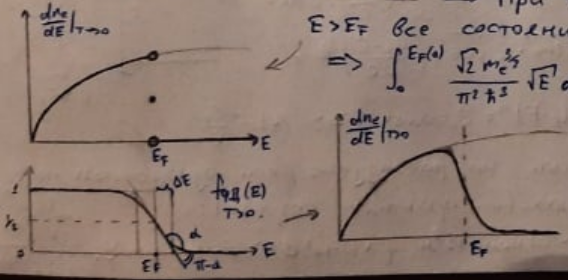
\includegraphics[width=.9\linewidth]{img/oral-04/oral-04-distribution-of-free-electrons.png}
  \caption{Графики распределения свободных электронов.
  График распределения при $T \to 0$ (слева-сверху).
  График распределения при увеличении температуры (справа).
  Графическое описания нахождения размытия уровня Ферми (слева-снизу)}
  \label{fig:free-electrons}
\end{figure}

\subsubsection{Оценка величины "размытия уровня Ферми" при $0 < kT \ll E_F$}

Продолжением анализа прошлого результата (про распределение свободных электронов) является анализ
того, что происходит с распределением при увеличении температуры. Так как при выполненом соотношении
$0 < kT \ll E_F$ график слабо отличается от графика при $T \to 0$ вне некоторого интервала
шириной $\Delta E$ вокруг точки $E_F$, ширину этого интервала можно оценить графически:
провести касательную к графику в точке $E_F$ (учитывая, что $dn_E / dE (E_F) = 1/2$):
\[
  |\tg (\pi - \alpha)| = \dfrac{1/2}{\Delta E} = \dfrac{1}{2 \Delta E}, 
  |\tg (\pi - \alpha)| = |\tg \alpha| = \left( \dfrac{d f_\text{Ф-Д}}{dE} \right)_{E = E_F} = \dfrac{1}{4kT}
  \Rightarrow \Delta E \approx 2kT
\]

\subsubsection{Влияние напряженности электрического поля на процесс ТЭЭ}
\label{sec:o244}
Cм. раздел \ref{sec:w7}. Если прикладывать напряжение между катодом и анодом, то работа
выхода металла будет смещаться. Причём приложим его в таком направлении, что
электроны будут притягиваться к аноду. Это приведёт к уменьшению $A_B$. Ключевым вопросом
является то, насколько изменится работа выхода внутри некоторого электрического поля.
Рассмотрим электрон, который вылетел с поверхности металла. Сила, с которой металл
притягивает его назад может быть найдена с помощью метода изображений. Согласно этому
методу, сила, действующая на заряженную частицу со стороны проводящей поверхности на расстоянии $x$,
равна силе, действующей между этой частицей и такой же, но с другим знаком на расстоянии $2x$:
$F_\text{из} = - \dfrac{k e^2}{(2x)^2}$. Потенциальная энергия такого
взаимодействия будет равна:
\[
  U_\text{из} = \int_x^{+\infty} F_\text{из} (t) \, dt
  =  - \dfrac{k e^2}{4 x}
\]
приложим теперь внешнее электрическое поле с напряженностью $\vec{\varepsilon}$, способствующее
выходу электронов из металла: $U_e = - e \varepsilon x, \vec{F} = - e \vec{\varepsilon}$.
Тогда общий потенциал:
\[
  U(x) = U_0 - e \varepsilon x - \dfrac{k e^2}{4 x} = U_0 - \alpha x - \dfrac{\beta}{x}.
\]
найдём максимум потенциальной энергии:
\[
  \dfrac{\partial U}{\partial x} (x_0) = 0 \Leftrightarrow x_0 = \sqrt{\dfrac{\beta}{\alpha}},
\]
и тогда значение изменения работы выхода будет:
$\Delta A_B = U_0 - U(x_0) = 2 \sqrt{\alpha \beta} = e^{3/2} k^{1/2} \varepsilon^{1/2}$,
тогда ток насыщения:
\[
  J_{x, \varepsilon}
  = const T^2 e^{-\dfrac{A_B - \Delta A_B}{kT}}
  = const T^2 e^{-\dfrac{A_B}{kT}} e^{ \dfrac{e^{3/2} k^{1/2} \varepsilon^{1/2}}{kT} }
  \Leftrightarrow
  \ln J_{x, \varepsilon}
  = const_1 + const_2 \varepsilon^{1/2}
\]
то есть ток будет увеличиваться и работа выхода будет уменьшаться.
На рисунке \ref{fig:shottki} приведена графическая иллюстрация.

\begin{figure}[H]
  \centering
  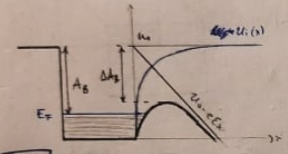
\includegraphics[width=.9\linewidth]{img/oral-04/Shottki.png}
  \caption{График потенциала $U_i$ до приложения внешнего поля (строго монотонный график,
  асимптота к которому горизонтальная линия);
  график потенциала после приложения внешнего поля (горка, асимптота -- прямая наклонная линия $U_0 = - e \varepsilon x$)}
  \label{fig:shottki}
\end{figure}


\subsubsection{Особенности зонной структуры легированных полупроводников. Оценка величины <<энергии ионизации>> примесных уровней}

\textit{Легирование полупроводников} — внедрение небольших количеств примесей или структурных дефектов с целью контролируемого изменения электрических свойств полупроводника.

см. Алексеев экзамен \#4
Примеси бывают разные. Они приводят к появлению избыточного количества или сво-
бодных электронов, или дырок. Их называют соответственно \textit{донорными} примесями (отдаю-
щими электроны) или \textit{акцепторными} примесями (забирающими электроны).

Соответственно легированные проводники бывают двух типов в зависимости от примесей, которые в них добавили:
\paragraph{Донорные полупроводники} 
В таких п/п избыток положительных свободных носителей заряда.

Донорные полупроводники -- получаются при добавлении в полупроводник элементов, от которых легко <<отрывается>> электрон.

Электроны в \textit{донорном} полупроводнике принято называть \textit{основными носителями заряда}, а дырки -- \textit{неосновными носителями заряда}.
\begin{figure}[H]
	\begin{minipage}{0.48\textwidth}
		\centering
		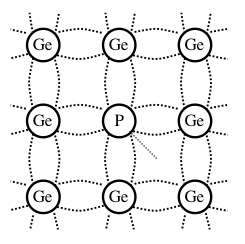
\includegraphics[width=0.7\linewidth]{img/oral-04/donor_poluprovodnik}
		\caption{Пример донорного полупроводника}
		\label{fig:donorpoluprovodnik}
	\end{minipage}\hfill
	\begin{minipage}{0.48\textwidth}
		\centering
		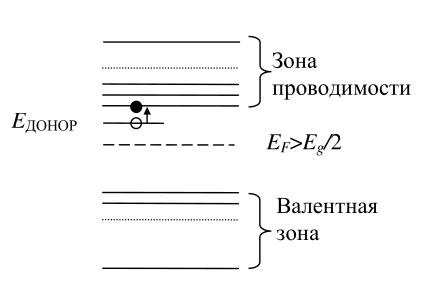
\includegraphics[width=\linewidth]{img/oral-04/donor_poluprovodnik1_energy}
		\caption{Энергетические уровни донорнрго полупроводника}
		\label{fig:donorpoluprovodnik1energy}
	\end{minipage}
\end{figure}
С точки зрения зонной теории наличие «легко отрывающихся» электронов соответствует появлению в запрещенной зоне донорных уровней энергии вблизи нижнего края зоны проводимости.

Уровень Ферми в донорном полупроводнике смещается вверх по шкале энергии, причем это смещение больше при низких температурах, когда концентрация свободных электронов значительно превышает число дырок. При повышении температуры, когда донорный характер полупроводника становится все менее и менее выраженным, уровень Ферми смещается в среднюю часть запрещенной зоны, как в беспримесном полупроводнике.
	
\paragraph{Акцепторные (дырочные, p-типа) полупроводники}
Получаются при добавлении в полупроводник элементов, которые легко <<отбирают>> электрон у атомов полупроводника. 
В таком случае в кристалле образуется избыток дырок.

Дырки в \textit{акцепторном} полупроводнике принято называть \textit{основными носителями}, а электроны - \textit{неосновными}.
\begin{figure}[H]
	\begin{minipage}{0.48\textwidth}
		\centering
		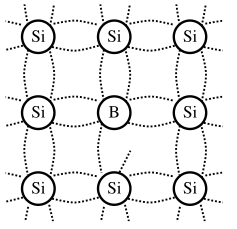
\includegraphics[width=0.7\linewidth]{img/oral-04/acceptor_poluprovodnik}
		\caption{Пример акцепторного полупроводника}
		\label{fig:acceptorpoluprovodnik}
	\end{minipage}\hfill
	\begin{minipage}{0.48\textwidth}
		\centering
		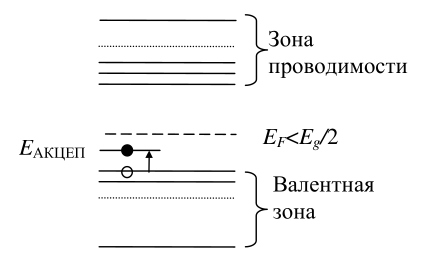
\includegraphics[width=\linewidth]{img/oral-04/acceptor_poluprovodnik1_energy}
		\caption{Энергетические уровни акцепторного полупроводника}
		\label{fig:acceptorpoluprovodnik1energy}
	\end{minipage}
\end{figure}

На языке зонной теории переход электрона из полноценной ковалентной связи в связь с недостающим электроном соответствует появлению в запрещенной зоне акцепторных уровней вблизи нижнего края зоны проводимости. Электрону для такого перехода из валентной зоны на акцепторный уровень требуется меньше энергии, чем для перехода из валентной зоны в зону проводимости, то есть для <<полного ухода>> электрона из ковалентной связи.

Уровень Ферми в акцепторном полупроводнике смещается вниз по шкале энергии, причем это смещение больше при низких температурах, когда концентрация дырок значительно превышает концентрацию свободных электронов. При повышении температуры, когда акцепторный характер полупроводника становится все менее и менее выраженным, уровень Ферми смещается в среднюю часть запрещенной зоны, как в беспримесном полупроводнике.

\paragraph{Энергия ионизации} --- энергия, которая необходимая для освобождения примесного электрона или дырки из примесного уровня. 

Для донорного полупроводника она отсчитывается от дна зоны проводимости до примесного уровня, а для акцепторного - от потолка валентной зоны по примесного уровня (см. Рис. \ref{fig:donorpoluprovodnik1energy} и \ref{fig:acceptorpoluprovodnik1energy}).

По значении энергии ионизации примесь делится на мелкую и глубокую. Если энергия ионизации примеси близка к половине ширины запрещенной зоны, то такую примесь называют глубокой. Если энергия ионизации примеси близка к уровню разрешенной зоны (реально меньше 0,1-0,05 еВ), то такую примесь называют мелкой. Чем больше энергия ионизации примеси, тем при той же температуре меньше концентрация свободных носителей заряда.

\subsubsection{Строение p-n перехода. Распределение объемного заряда, концетраций дырок и электронов, электрического потенциала. Вывод формулы Шокли}

$p-n$ нереходом называют тонкий слой, образующийся в месте контакта двух областей полупроводников
акцепторного и донорного типов. С одной стороны от перехода будет область $p$ типа, в которой
основным носителем заряда будут дырки, с другой стороны -- область $n$ типа, в которой основными
носителями заряда будут электроны. В области контакта полупроводников носители заряда будут
проходить через переход, вызывая <<рекомбинацию>> -- то есть взаимное <<уничтожение>> электрона и дырки.
За счёт этого вблизи границы концентрация обоих носителей близка к нулю.

Из-за распределения зарядов примесных ионов в зоне контакта возникает контактное электрическое поле,
которое "противодействует" переходу основных носителей через границу контакта. Это приводит к возникновению потенциального барьера высоты $U_0$, кроме того, подключённый источник гапряжения изменяет высоту потенциального барьера: повышает, если минус источника подключён к p-области.

В равновесном состояниии $j_\text{ОСН} = j_\text{НЕОСН}$, $j_\text{ОСН} = j_0 \cdot e^{-\dfrac{U_0}{kT}}$, а полный ток $j = j_\text{ОСН} - j_\text{НЕОСН} = 0$.

Если прикладывается напряжение $V>0$, то $j_\text{ОСН} = j_0 \cdot e^{-\dfrac{U_0-eV}{kT}}$, следовательно, $j = j_\text{ОСН} - j_\text{НЕОСН} = j_0 e^{-\dfrac{U_0-eV}{kT}} - j_0 \cdot e^{-\dfrac{U_0}{kT}} = j(T) \cdot \left( e^{\dfrac{eV}{kT}} - 1 \right) $ - формула Шокли.

\subsubsection{Эффект Холла в полупроводнике с двумя типами носителей заряда}

Рассмотрим полупроводник, находящийся в магнитном поле $\vec{B}$ и в электрическом поле
$\vec{E}_{||}$.  Концентрации и подвижности носителей зарядов обозначим $n_e, n_h, \mu_e, \mu_h$.
Скорость дрейфа обозначим $\vec{v}_d$. Для скорости дрейфа раннее (вопрос 10, равенство
\eqref{write:10:v_d}) было получено соотношение $\vec{v}_d = \mu \vec{E}$.

\begin{figure}[H]
  \centering
  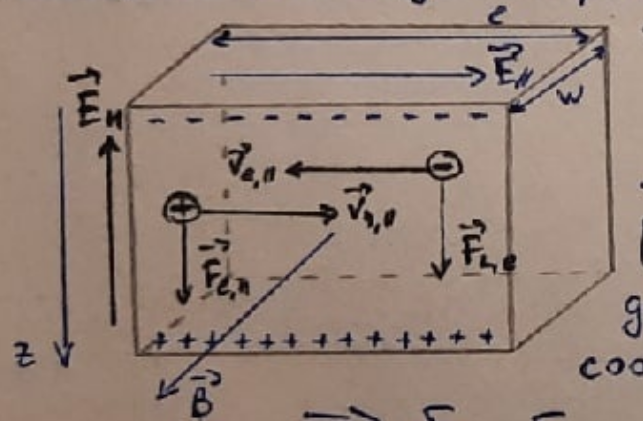
\includegraphics[width=0.9\linewidth]{img/oral-04/hall-effect.png}
  \caption{Иллюстрация эффекта Холла}
  \label{fig:halleffect}
\end{figure}

На заряды будет действовать сила Лоренца:
\[
  F_{L, h} = e \cdot v_{h, ||} \cdot B = e \mu_h E_{||} \cdot B,
  F_{L, e} = e \cdot v_{e, ||} \cdot B = e \mu_e E_{||} \cdot B,
\]
Согласно рисунку \ref{fig:halleffect}, при $\vec{E}_{||}$ направленном направо, дырки будут 
двигаться направо, при $\vec{B}$ направленном на нас, сила Лоренца на дырки будет действовать вниз,
соответственно, снизу будет накопление дырок, аналогично получаем, что сверху накопятся электроны.
Вследствие этого накопления появится напряженность Холла $\vec{E}_H$, направленная снизу вверх.
Сила, соответствующая этой напряженности в проекции на ось $z$:
\[
  F_{H, h, z} = -e E_{H}, \quad
  F_{H, e, z} = e E_{H}
\]
Тогда суммарная сила в проекции на ось $z$:
\[
  F_{h, z} = F_{L, h} + F_{H, h, z} = e \left( E_{||} B \mu_h - E_H \right); \quad
  F_{e, z} = F_{L, e} + F_{H, e, z} = e \left( E_{||} B \mu_e + E_H \right)
\]

В течение некоторого небольшого времени от начала эксперимента электроны и дырки будут перемещаться 
и скапливаться сверху и снизу. Рассмотрим плотность тока электронов, которые направляются к своей 
области скопления --- вверх, а также плотность тока дырок, направляющихся вниз:
\begin{align*}
  j_{+, e} &= q \cdot n \cdot v_d
    = -e \cdot n_e \cdot \dfrac{F_{e, z}}{e} \cdot \mu_e
    = -e n_e \mu_e (E_{||} B \mu_e + E_H); \\
  j_{+, h} &= q \cdot n \cdot v_d
    = e \cdot n_h \cdot \dfrac{F_{h, z}}{e} \cdot \mu_h
    = e n_h \mu_h (E_{||} B \mu_h - E_H),
\end{align*}
здесь у нас дрейфовая скорость понимается в смысле усреднённой скорости в проекции на ось $z$. 
Поэтому здесь дрейфовая скорость вот такая: $\vec{v}_d = \mu \vec{E}= \mu \vec{F} / e$
\footnote{эта напряженность $\vec{E}$ понимается как <<эффективная>>, то есть это такая
напряженность, чтобы создавать такую силу $\vec{F}$, несмотря на то, что эта сила имеет природу
не как сила, создаваемая какой-то реальной напряженностью}.
По прошествии некоторого времени, всё устаканится и будет установившийся режим, то есть количество
электронов, приходящих наверх будет равно количеству дырок, приходящих вниз, а значит и плотности
тока будут равны по модулю, а значит можно записать:
\begin{multline*}
  j_{+, e} + j_{+, h} = 0
  \Rightarrow
  -e n_e \mu_e (E_{||} B \mu_e + E_H) + e n_h \mu_h (E_{||} B \mu_h - E_H)
  \Rightarrow \\
  \Rightarrow
  E_{||} B (n_h \mu_h^2 - n_e \mu_e^2) = E_{H} (n_e \mu_e + n_h \mu_h)
  \Rightarrow
  \dfrac{E_{H}}{E_{||}} = \dfrac{n_h \mu_h^2 - n_e \mu_e^2}{n_e \mu_e + n_h \mu_h} B
\end{multline*}

\paragraph{Предельные случаи}

\begin{align*}
  n_e &\gg n_h \Rightarrow \dfrac{E_{H}}{E_{||}} = \dfrac{- n_e \mu_e^2}{n_e \mu_e} B
  \Rightarrow E_{H} = - \mu_e B E_{||} \\
  n_h &\gg n_e \Rightarrow \dfrac{E_{H}}{E_{||}} = \dfrac{n_h \mu_h^2}{n_h \mu_h} B
  \Rightarrow E_{H} = \mu_h B E_{||}
\end{align*}
 \newpage
  \subsection{Ключевые эксперименты}

\subsubsection{Опыт Резерфорда по рассеянию $\alpha$-частиц}

\subsubsection{Измерение спектра излучения АЧТ}

\subsubsection{Фотоэффект}

\subsubsection{Комптон-эффект}

\subsubsection{Дифракция электронов (в чем отличие от дифракции рентгеновских лучей?)}
\begin{itemize}
  \item опыт Девисона-Джермера (монокристалл);
  \item Опыты Томсона  и Тартаковского (поликристалл);
  \item Опыт Фабриканта (одиночные электроны);
\end{itemize}

\subsubsection{Опыт Штерна-Герлаха}
 \newpage
  \subsection{Атомы, молекулы, строение вещества}

\subsubsection{Состав атома (электроны, ядра, нуклоны). Характеристики входящих в него частиц}

\subsubsection{Магнитный орбитальный момент. Магнетон Бора $\mu_B$ (вывод)}

Если рассматривать атом водорода с квантовым числом $n=0$, что говорит нам о том, что квантовое
число $m \in \left\{ 0 \right\} \Leftrightarrow m=0$, то есть $L_z = 0$. С точки зрения
классической механики, электрон движется
по круговой орбите радиуса $r$ с круговой частотой $\omega$. Сила тока: $I = \dfrac{dq}{dT}$.
За время $T = \dfrac{2\pi}{\omega}$ электрон полностью пройдёт по орбите, а значит $dq = e$, 
$I = \dfrac{e \omega}{2\pi}$. Магнитный момент, по определению, равен
$\vec{P}_m = \dfrac{I}{2} \oint [\vec{r}, \vec{dl}] = I S \vec{n}$, где S -- площадь
поверхности, замкнутой внутри контура, $\vec{n}$ -- нормаль к этой поверхности.
Получается, что $P_m = \dfrac{e}{T} \pi r^2 = \dfrac{e \omega r^2}{2}$. Момент импульса
выражается через магнитный момент: $\vec{L_z} = \vec{r} \times \vec{P}_m$,
$L = m_e vr = m_e \omega r^2$.
Гиромагнитным соотношением называется $\gamma = \dfrac{P_m}{L_z} = \dfrac{e}{2m_e}$. 
То есть $P_m = \gamma L_z = \dfrac{e \hbar}{2 m_e} m = \mu_\text{Б} m$, где $m$ -- орбитальное квантовое число.
Постоянная $\mu_B = \dfrac{e \hbar}{2 m_e}$ называется магнетоном Бора. Как видно, это 
своеобразная <<единица измерения>> магнитного момента. 

Но однако из эксперимента Штерна и Герлаха видно, что для атомов серебра с $m=0$ всё равно
почему-то магнитный момент ненулевой. Из этого Уленбек и Гаудемит выдвинули гипотезу о том, 
что у электрона есть свой собсвтенный механический момент, не связанный с его движением как целого,
то есть с движение его центра масс. Этот собственный механический момент называют спином.
А момент импульса, который добавляется -- $L_z^s$ называют спиновым механическим моментом.

Куча терминов:
\begin{itemize}
  \item $s$ -- спиновое квантовое число;
  \item $s_m$ -- пиновое магнитное квантовое число;
  \item $L_z^L, L_z^s$ -- орбитальный и спиновые моменты;
  \item $P_{mz}^s$ -- спиновый магнитный момент.
    Для него верно: $P_{mz}^s = 2 \mu_B \cdot s_m \in \left\{ -\mu_B, \mu_B \right\}$.
    Этот факт был получен экспериментально;
  \item $L_z = L_z^L + L_z^s$ -- полный;
  \item $L_z^L = \hbar m, m \in \left\{ 0, \pm 1, \pm 2, \dots, \pm l \right\}, l \in \left\{ 0, 1, \dots, n-1 \right\}$ -- орбитальный момент;
  \item $L_z^s = \hbar m_s, m_s \in \left\{ - \dfrac{1}{2}, \dfrac{1}{2} \right\}$ -- спиновый момент.
\end{itemize}

\end{document}
